\begin{apendicesenv}

% Imprime uma página indicando o início dos apêndices
\partapendices

% Para cada apêndice, um \chapter


% ==============================================================================
\chapter{Experiment 1 (EX1)}
% ==============================================================================

\begin{figure}
    \centering
    % 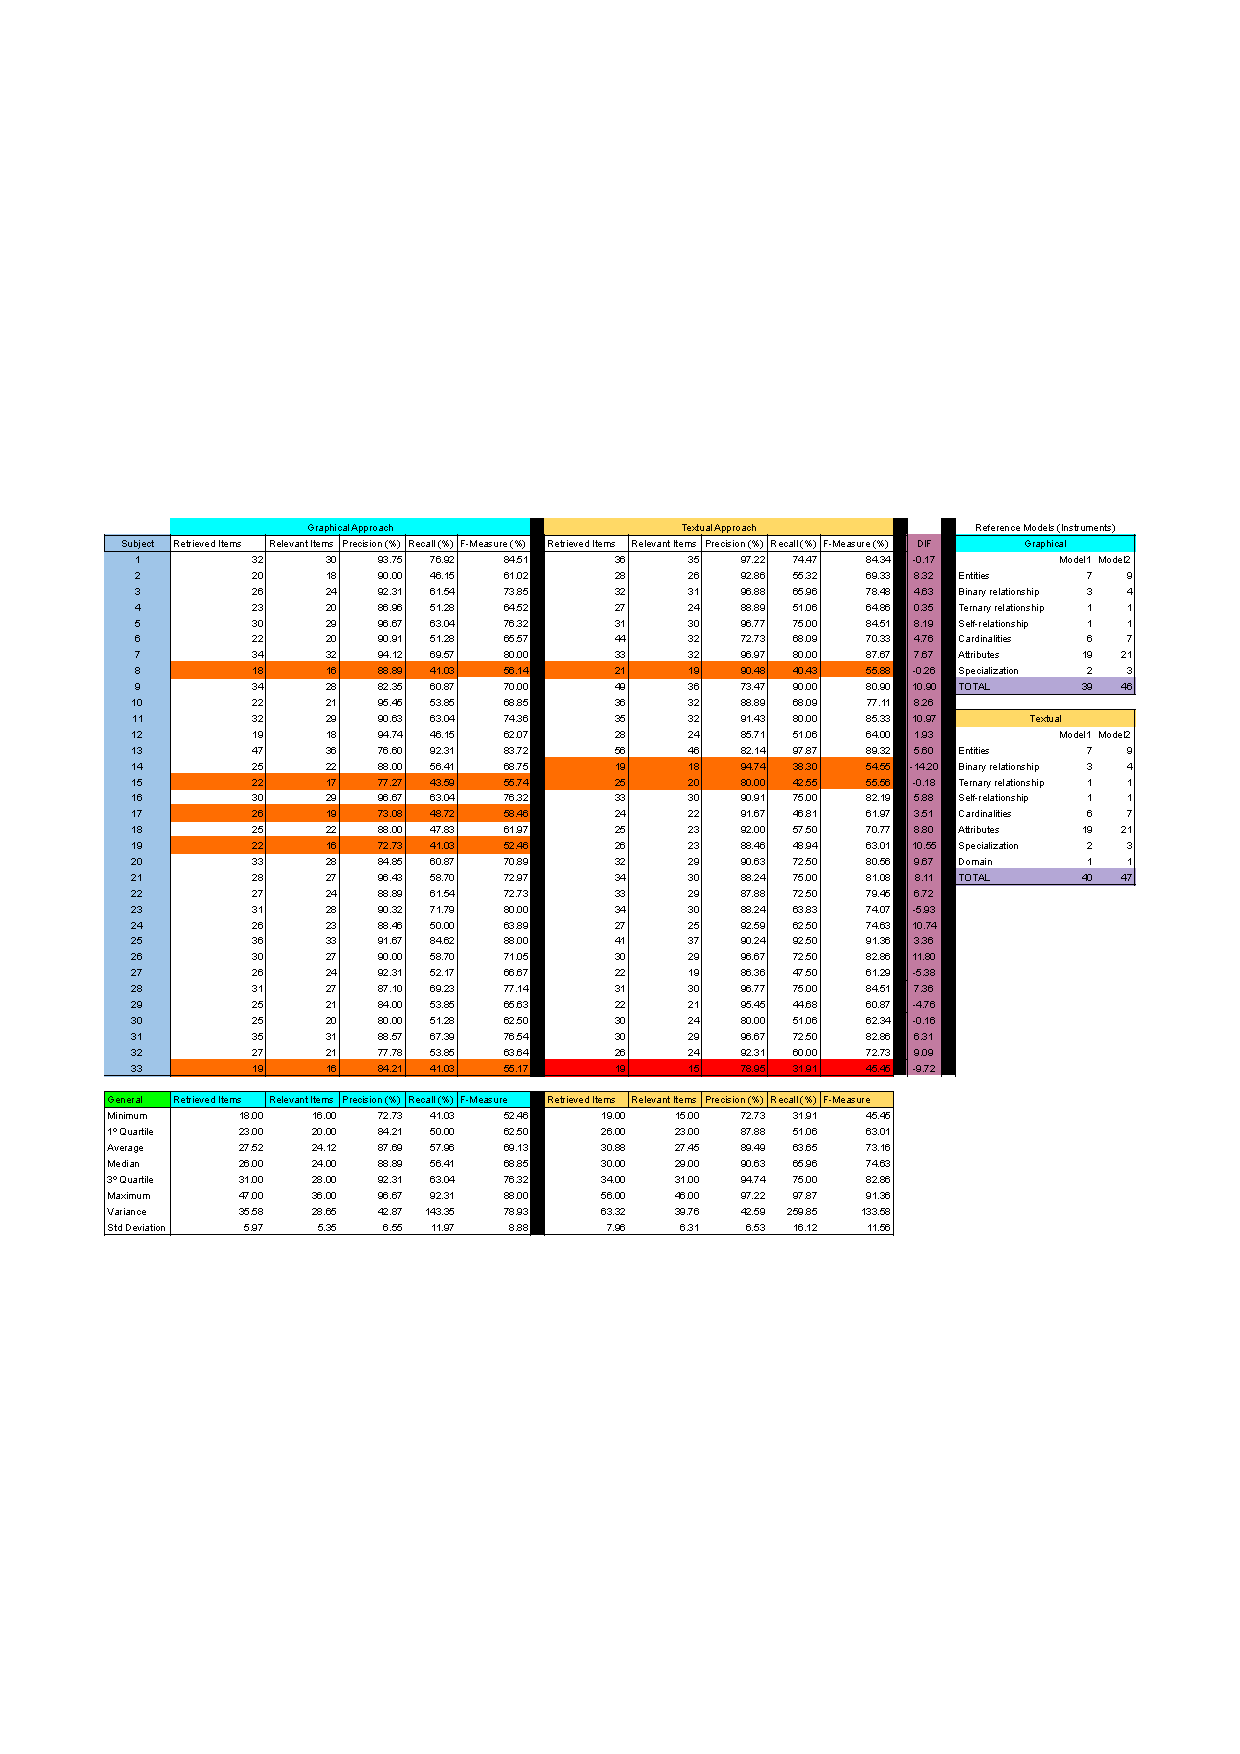
\includegraphics[]{postextuais/appendix/EX1-Results.pdf}
    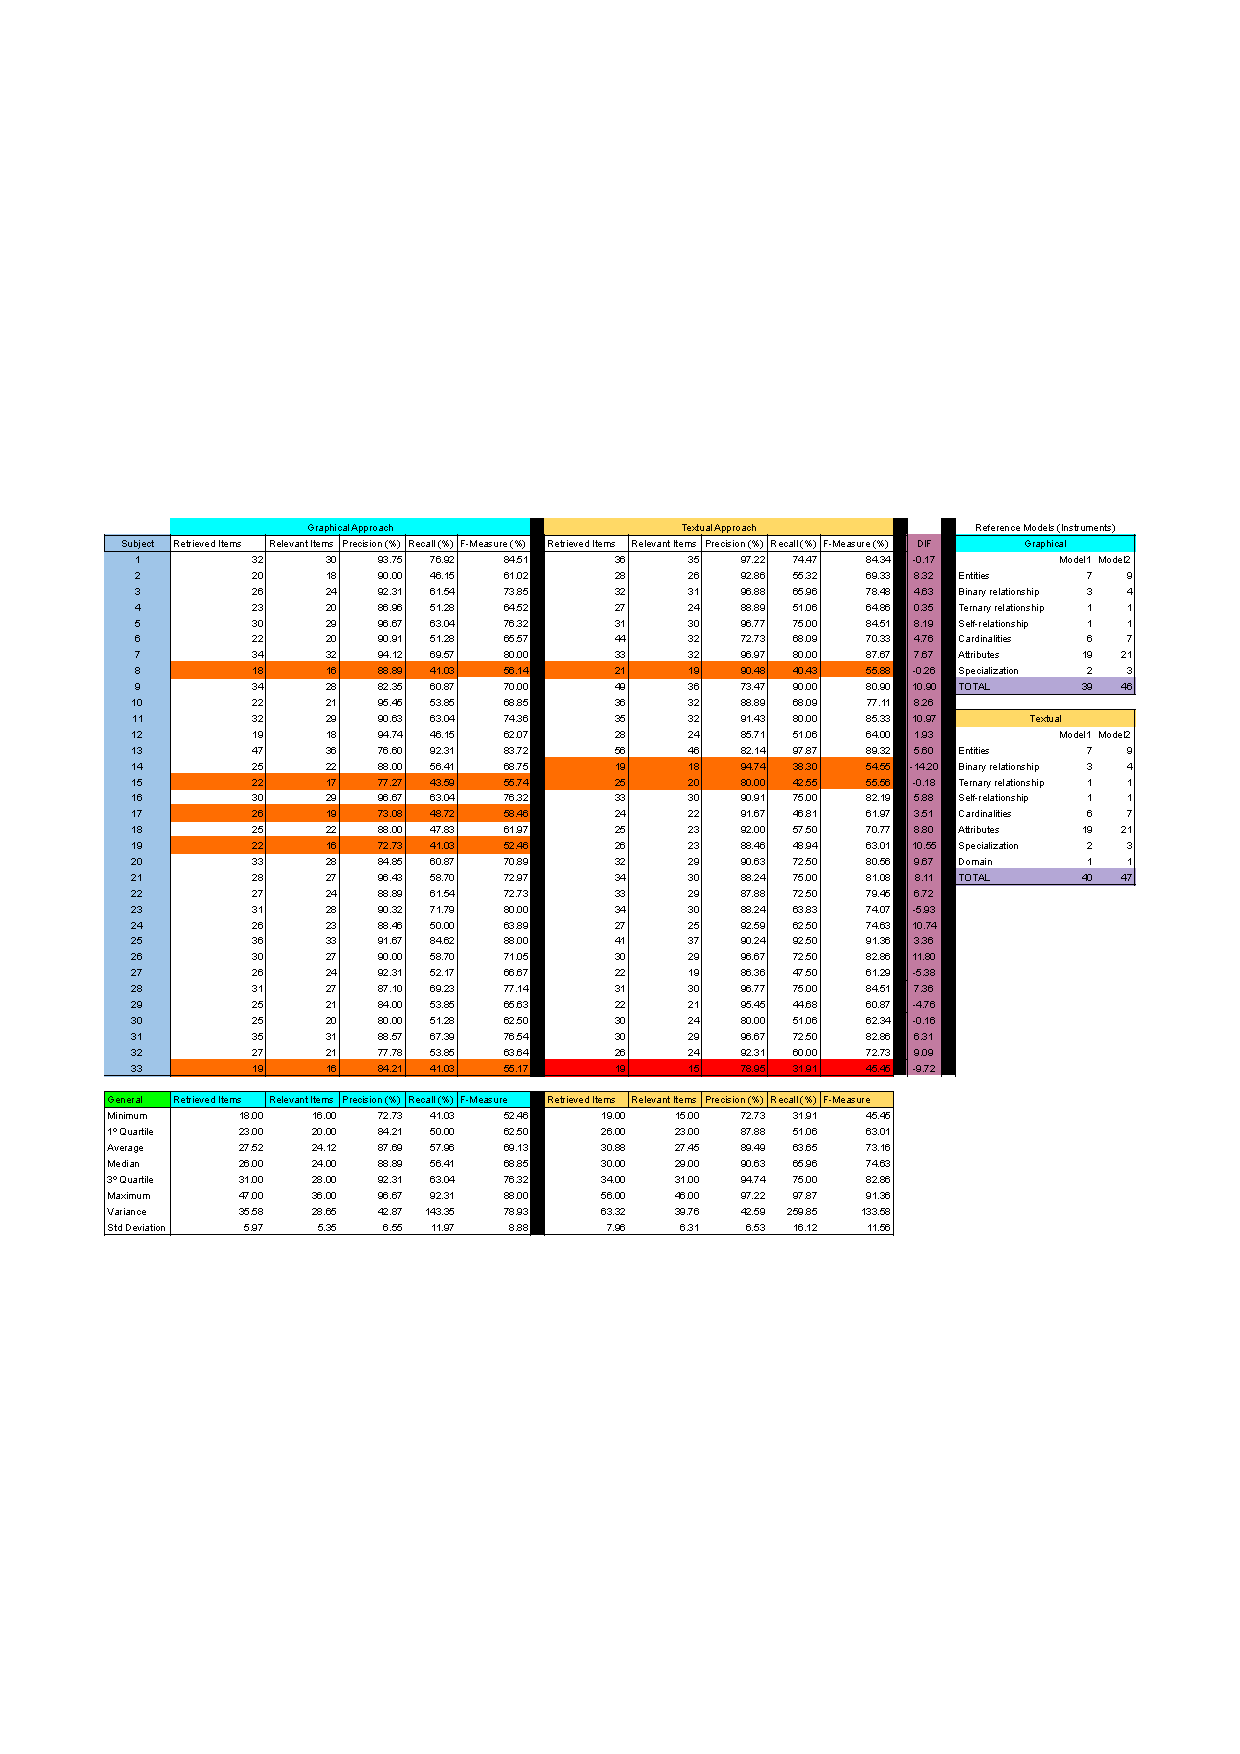
\includepdf[pages=-, frame=false, scale=0.90]{postextuais/appendix/EX1-Results.pdf}
    \caption{EX1 - F-Score.}
    \label{fig:ex1FScore}
\end{figure}

\newpage

\begin{figure}
    \centering
    % 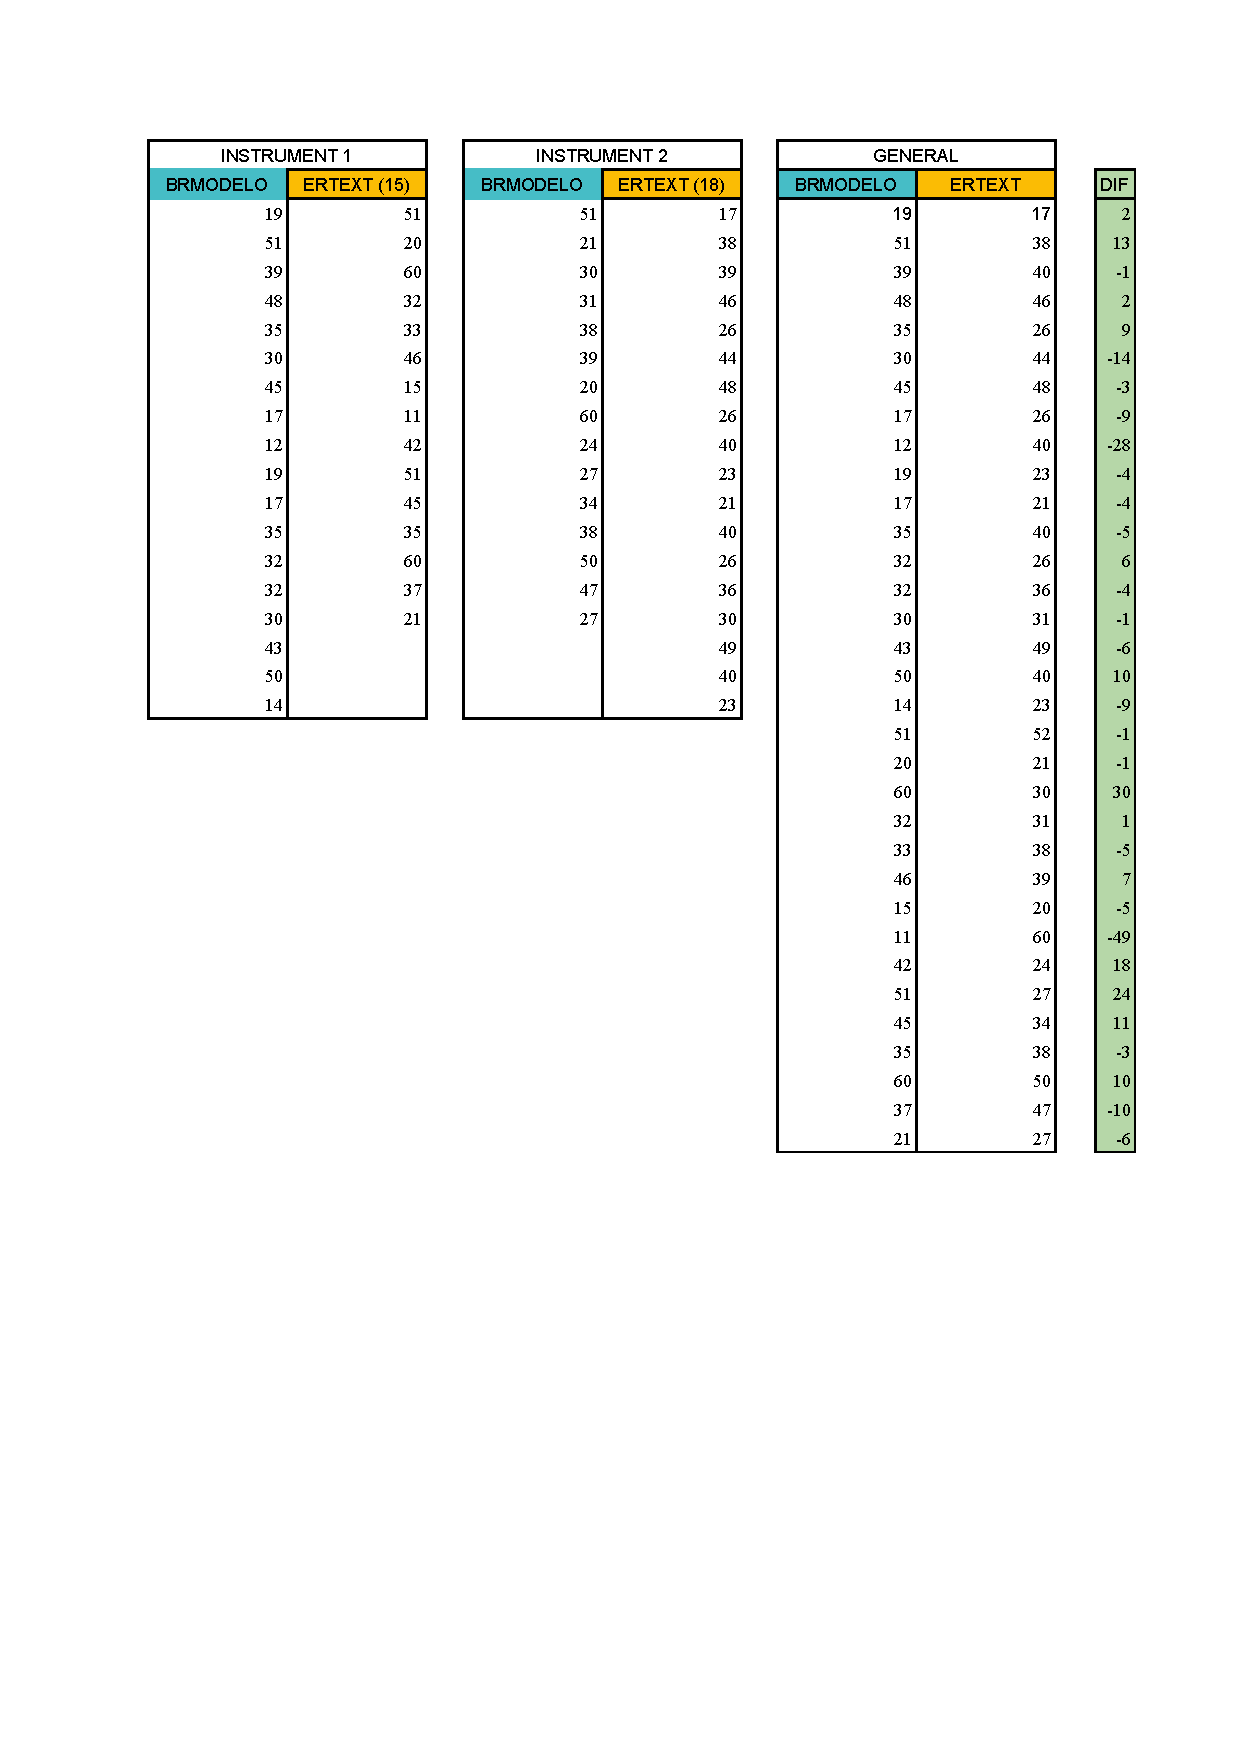
\includegraphics[]{postextuais/appendix/EX1-Results-Times.pdf}
    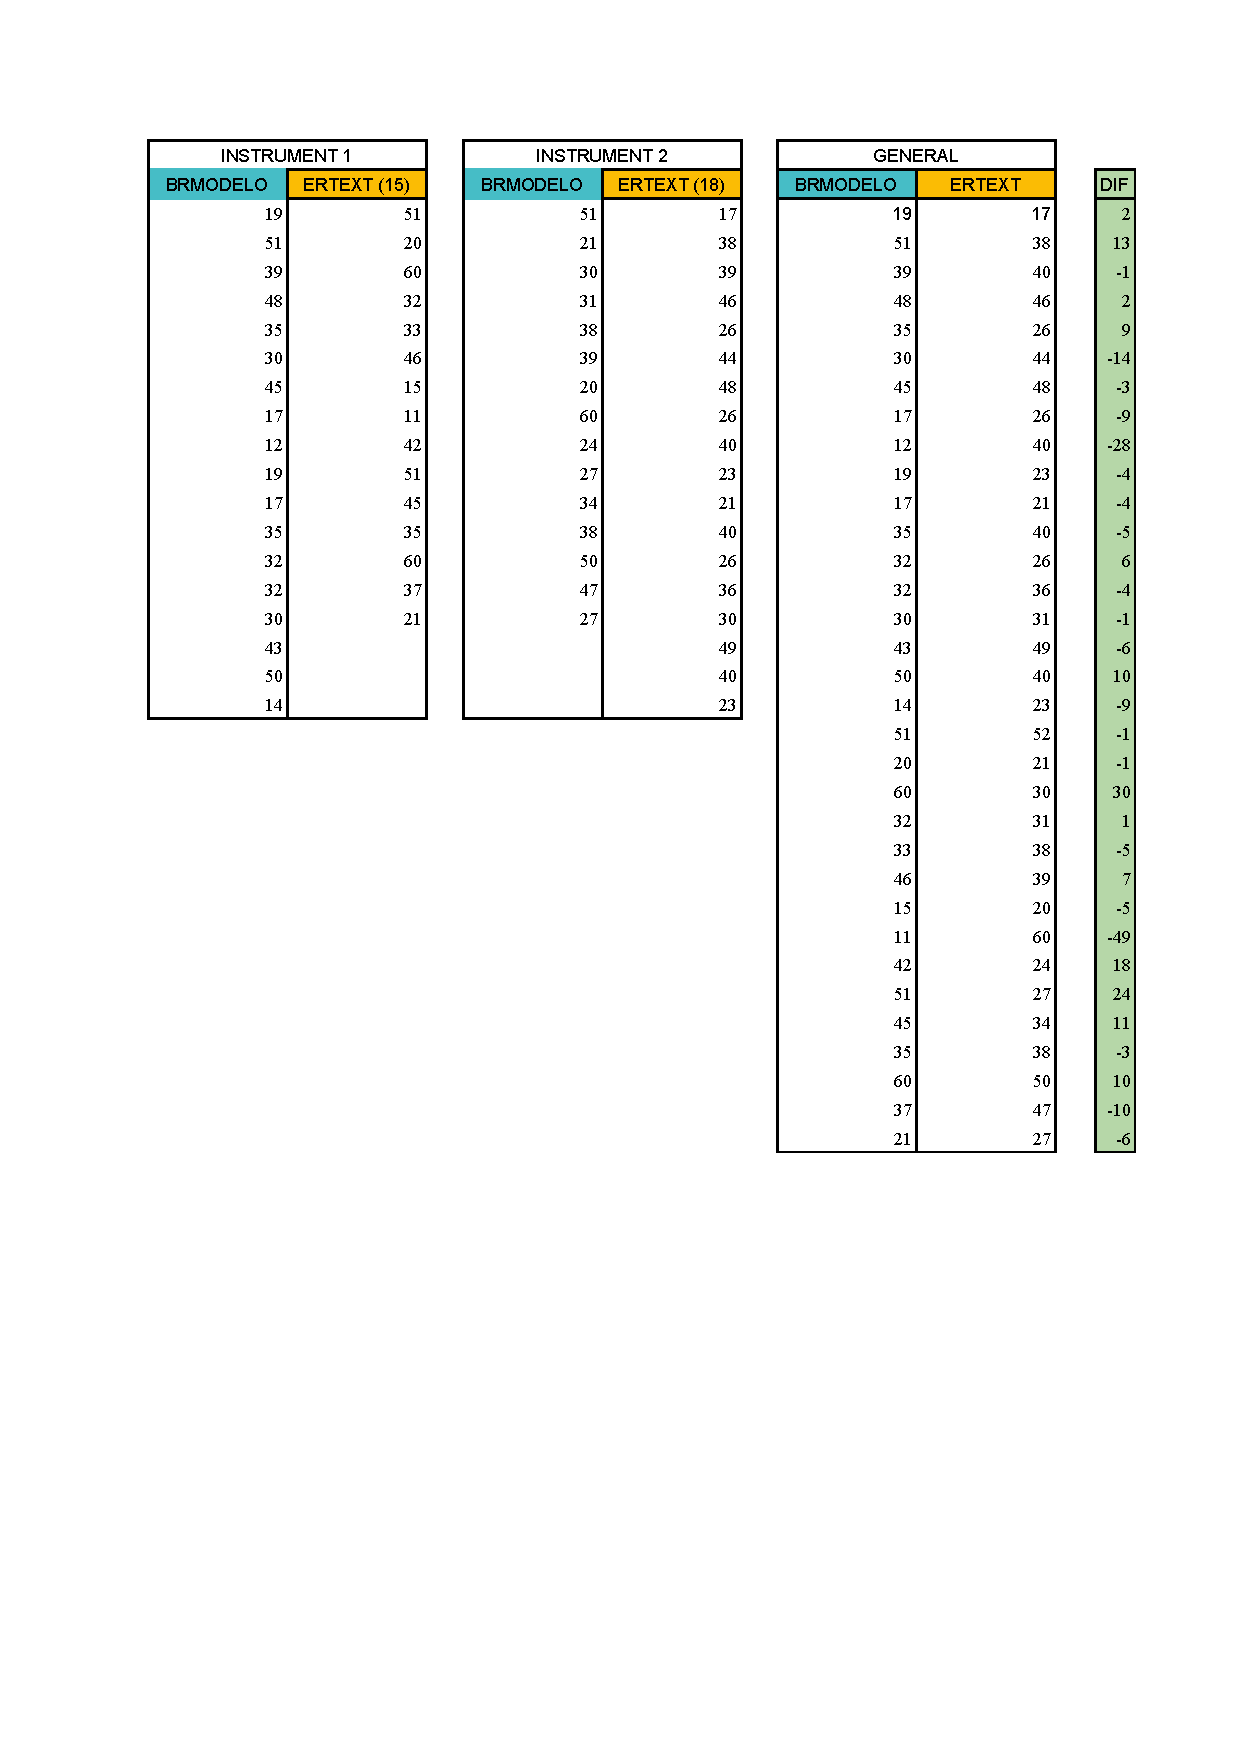
\includepdf[pages=-, frame=false, scale=0.90]{postextuais/appendix/EX1-Results-Times.pdf}
    \caption{EX1 - times.}
    \label{fig:ex1Times}
\end{figure}

% ==============================================================================
\chapter{Experiment 2 (EX2)}
% ==============================================================================

\begin{figure}
    \centering
    % 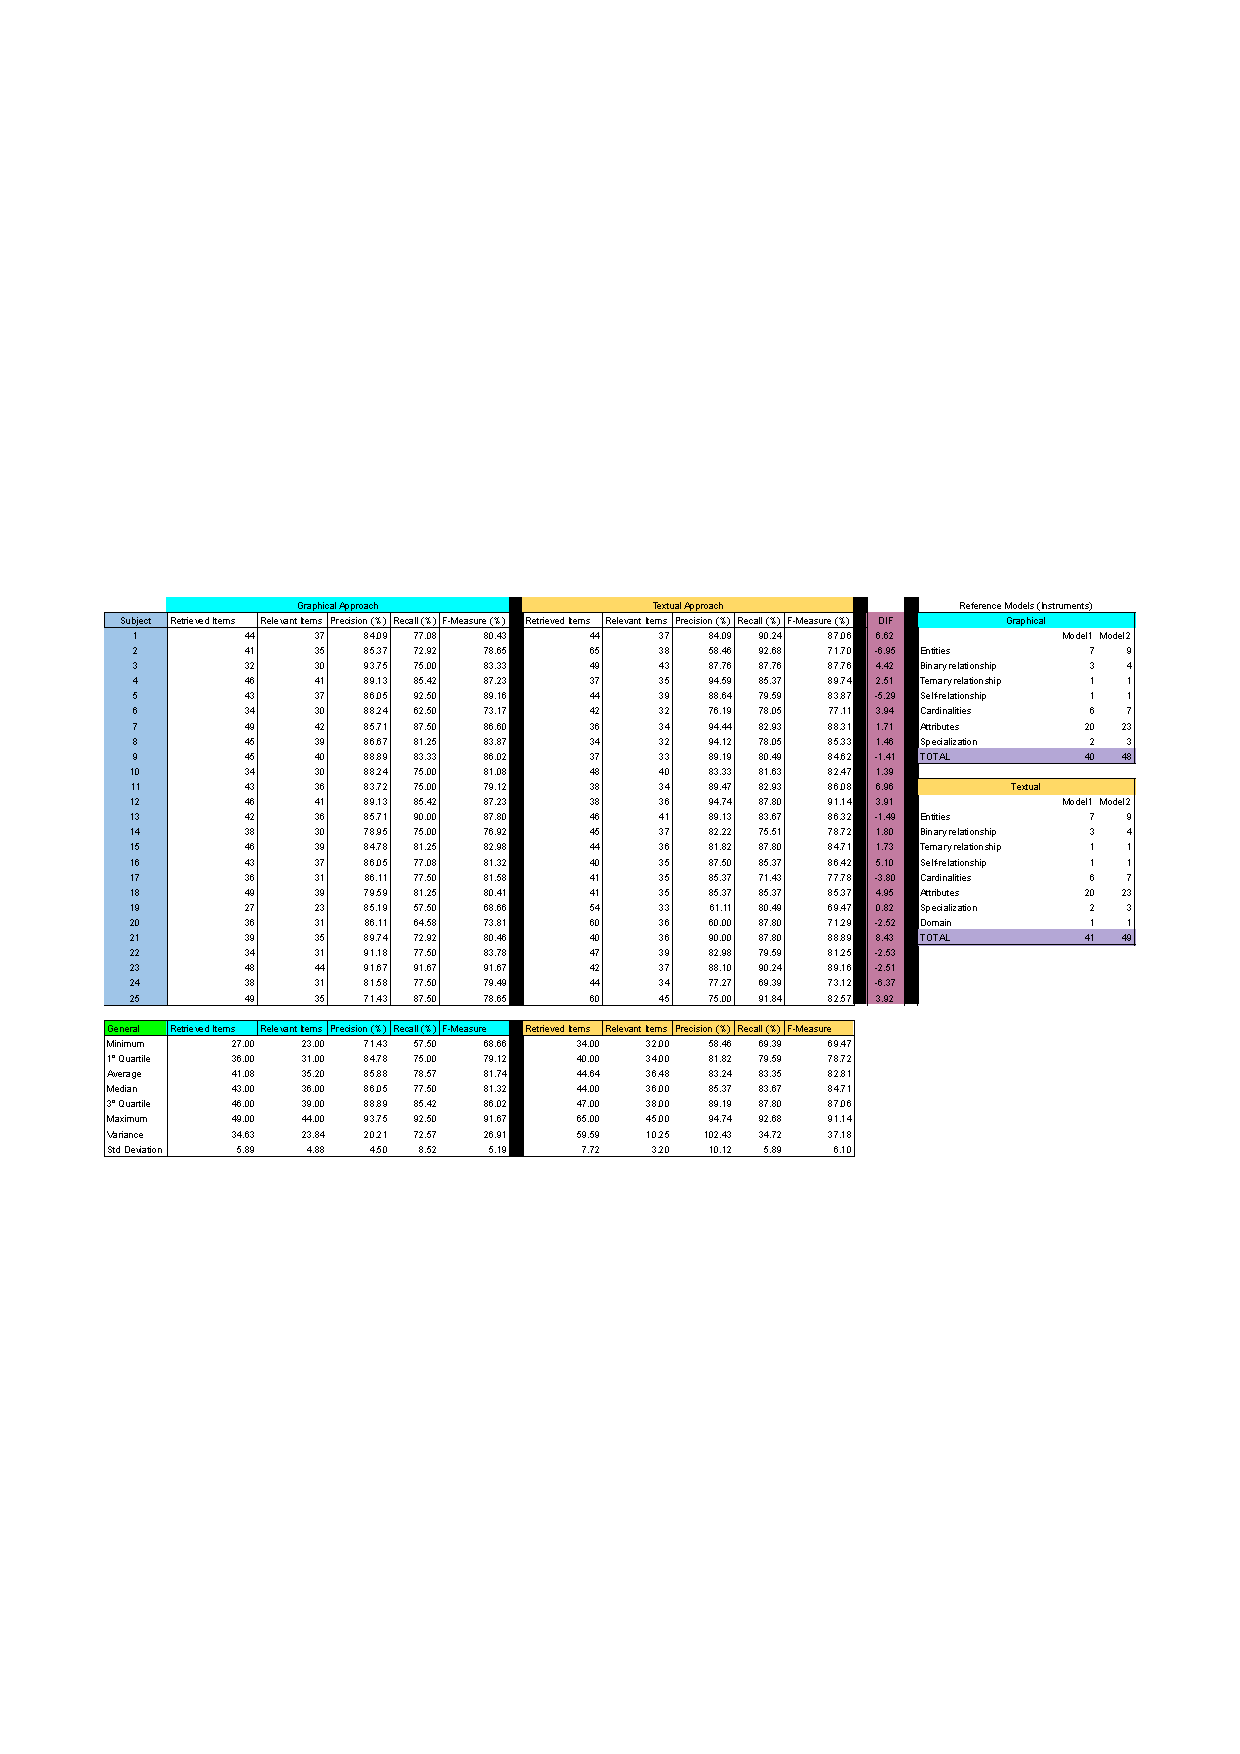
\includegraphics[]{postextuais/appendix/EX2-Results.pdf}
    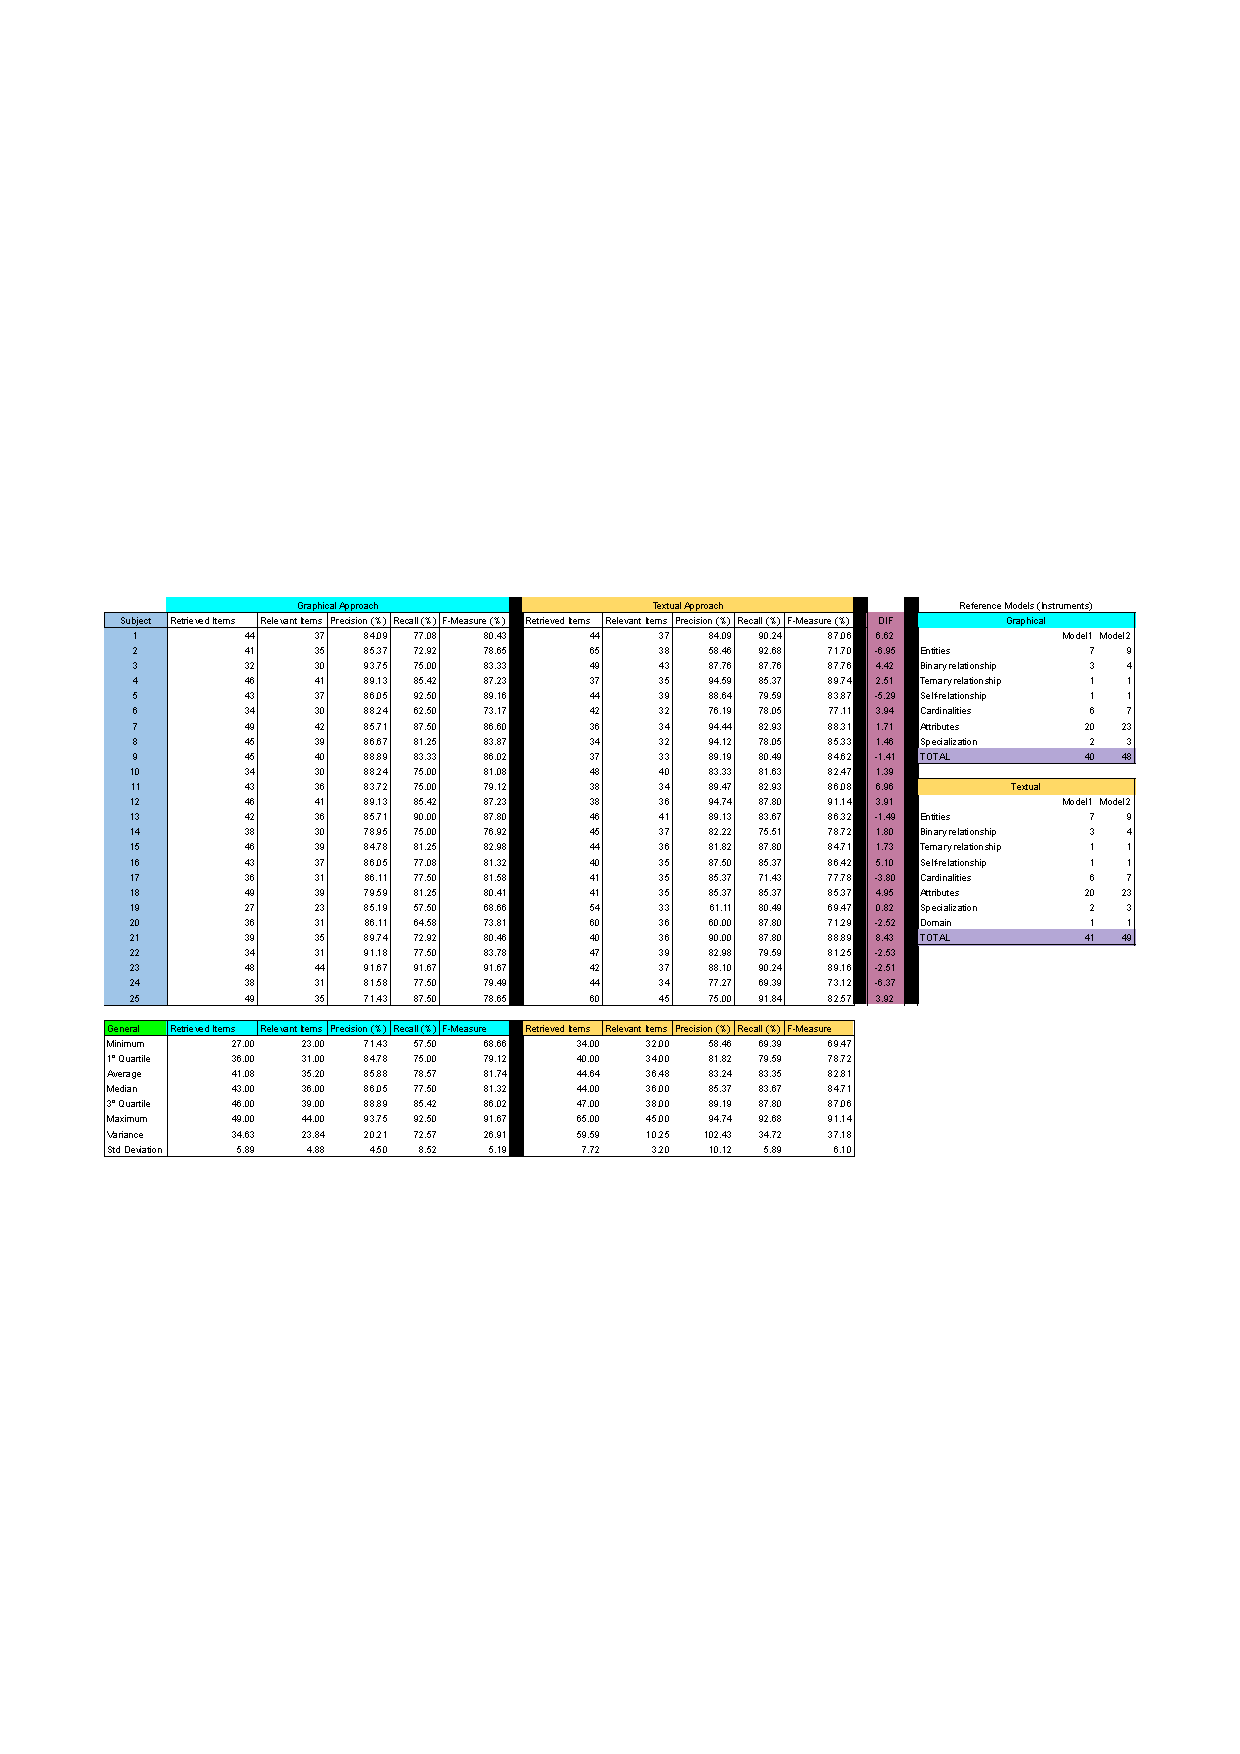
\includepdf[pages=-, frame=false, scale=0.90]{postextuais/appendix/EX2-Results.pdf}
    \caption{EX2 - F-Score.}
    \label{fig:ex2FScore}
\end{figure}

\newpage

\begin{figure}
    \centering
    % 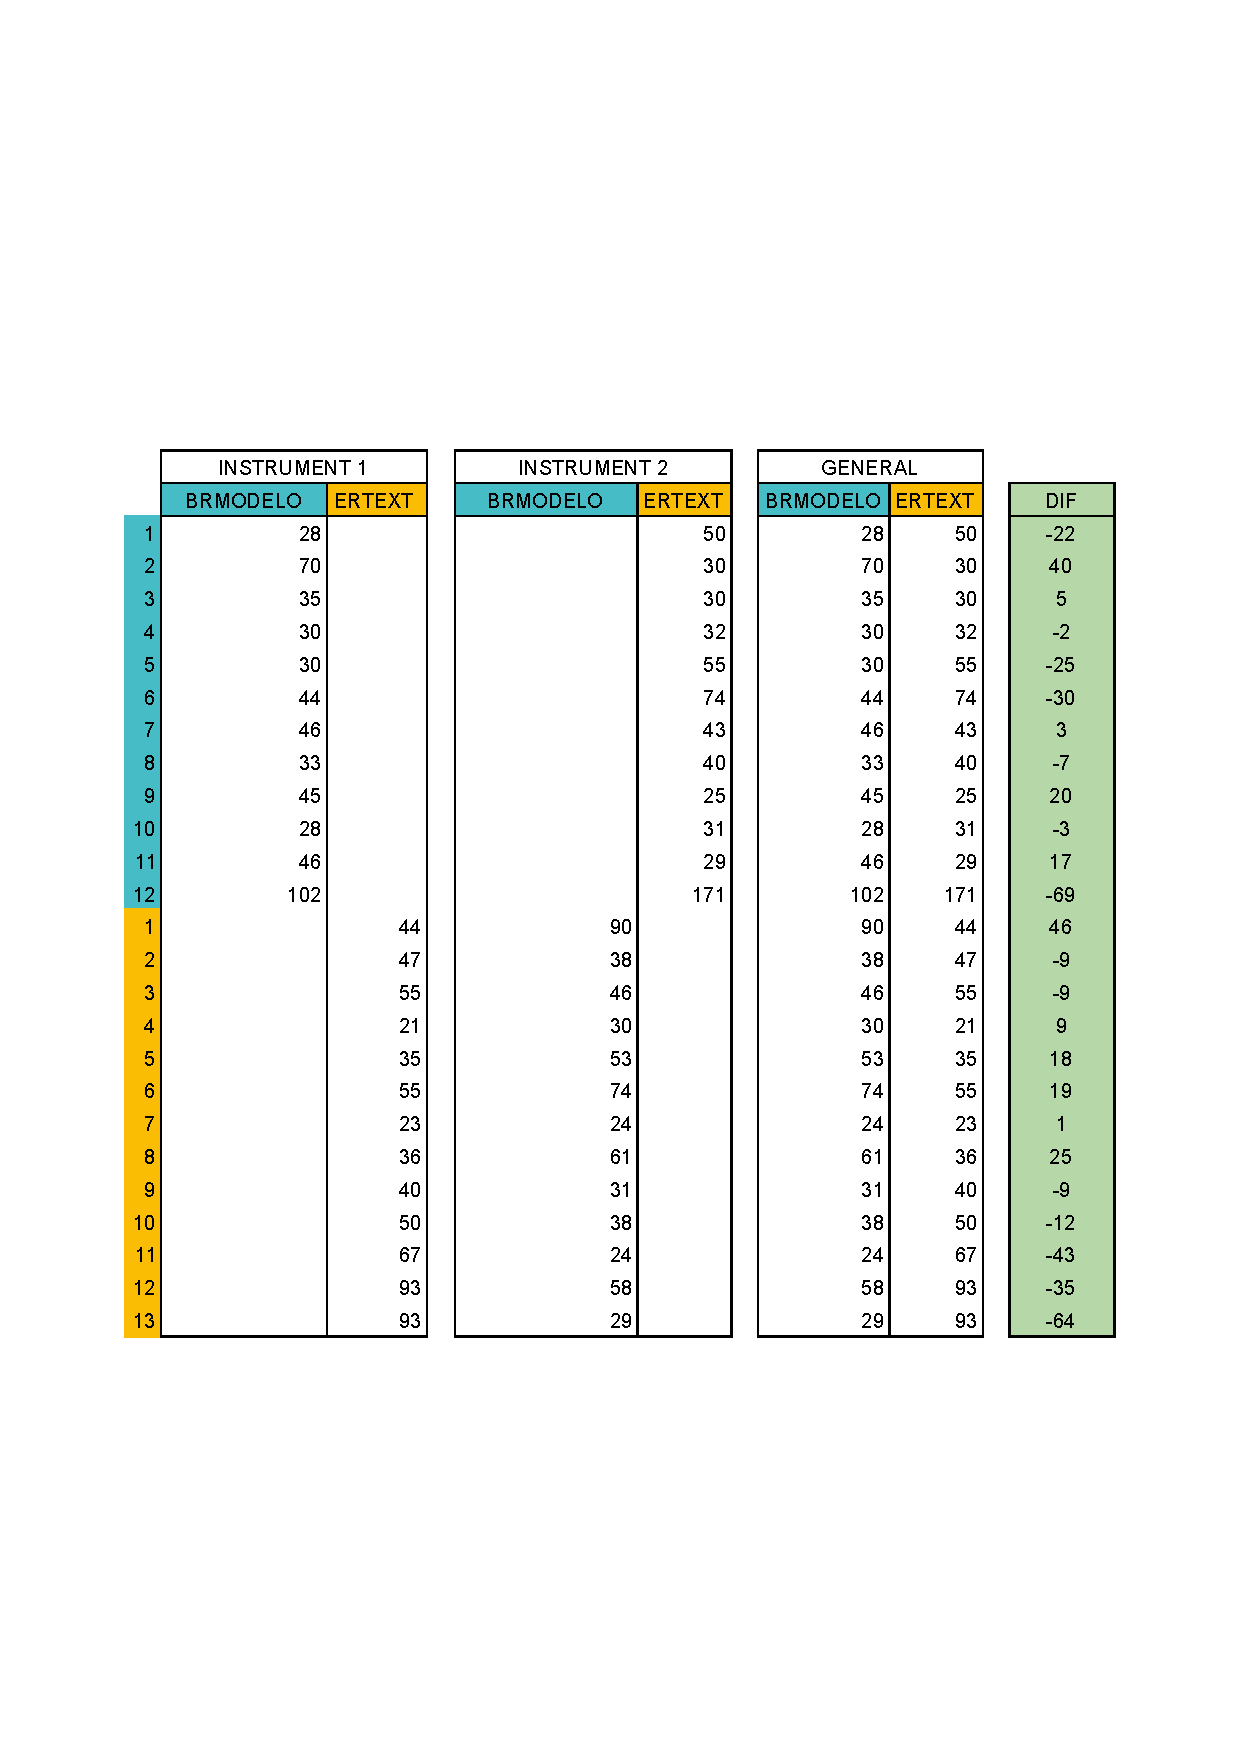
\includegraphics[]{postextuais/appendix/EX2-Results-Times.pdf}
    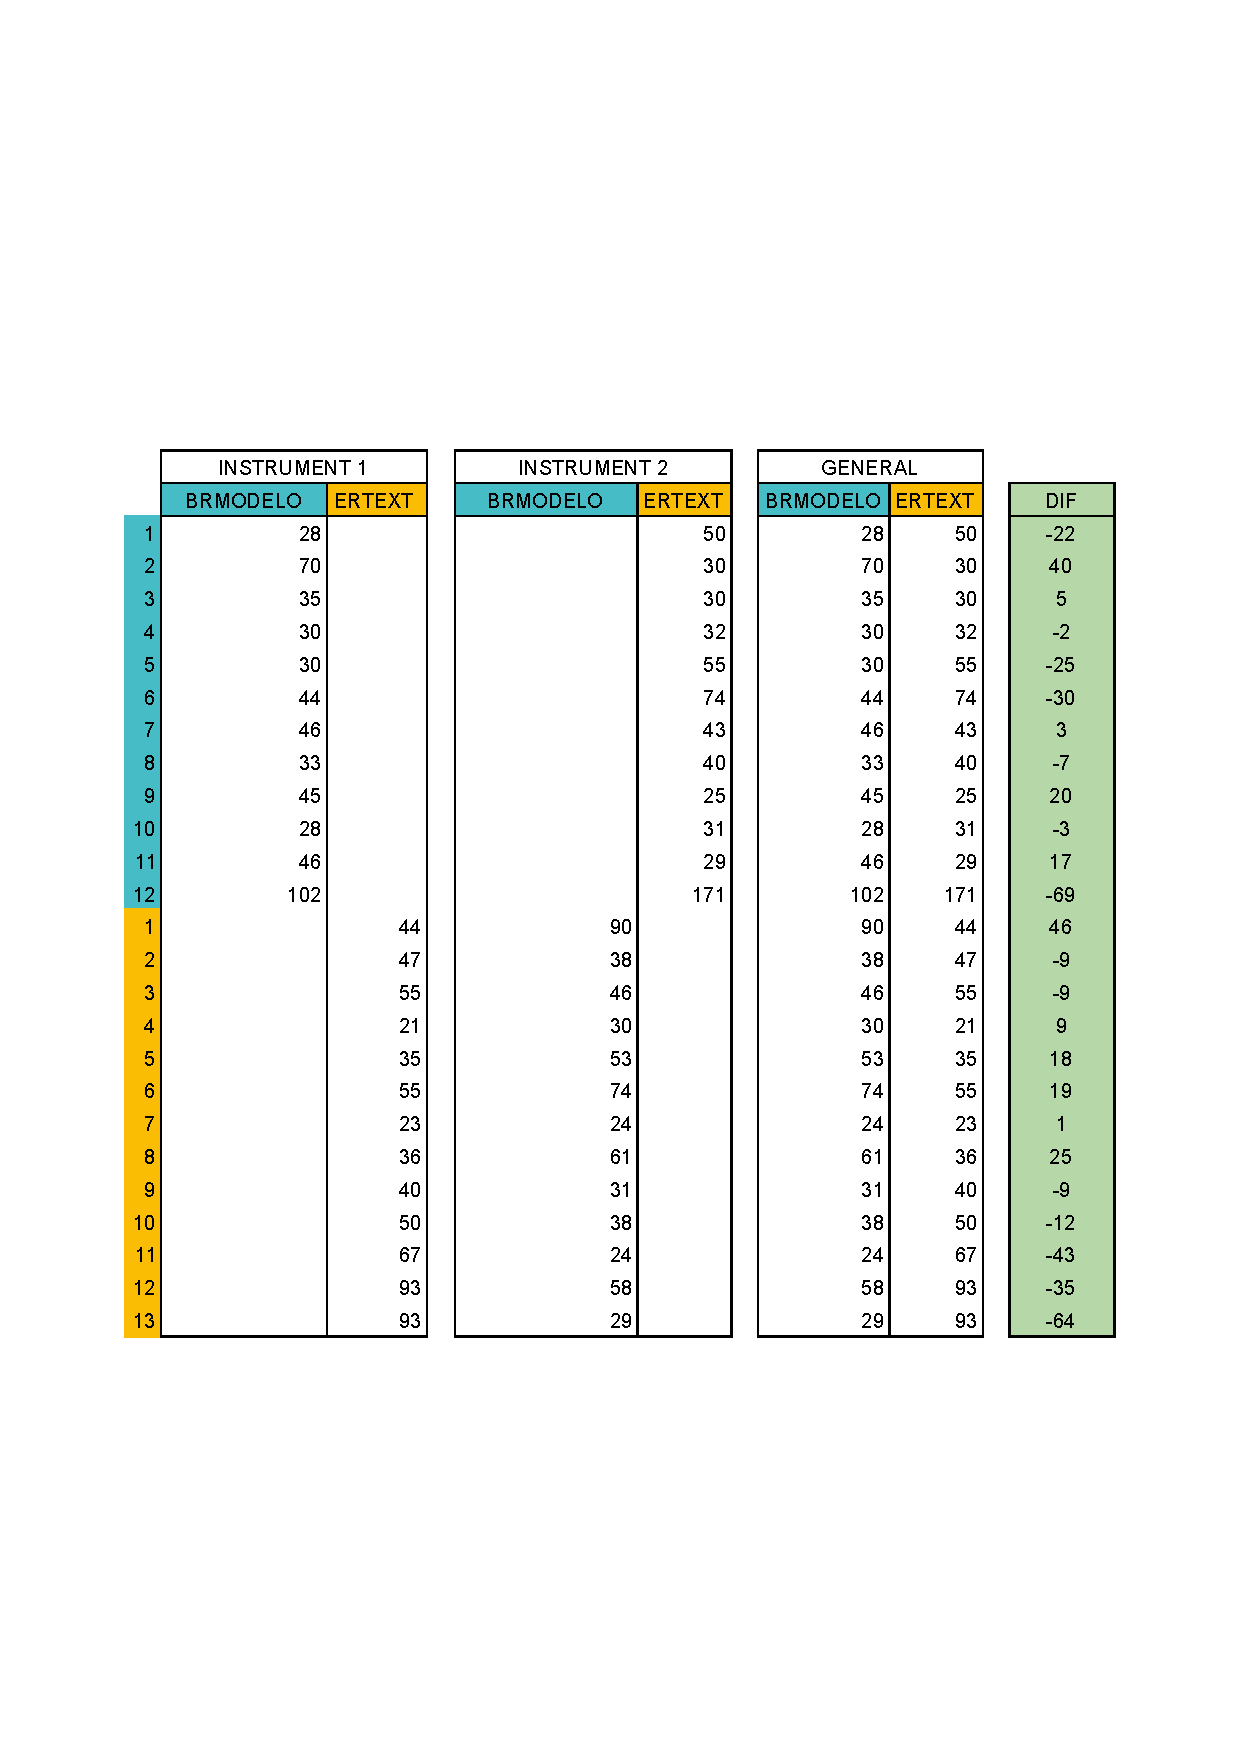
\includepdf[pages=-, frame=false, scale=0.90]{postextuais/appendix/EX2-Results-Times.pdf}
    \caption{EX2 - Times.}
    \label{fig:ex2Times}
\end{figure}

\newpage

\begin{figure}
    \centering
    % 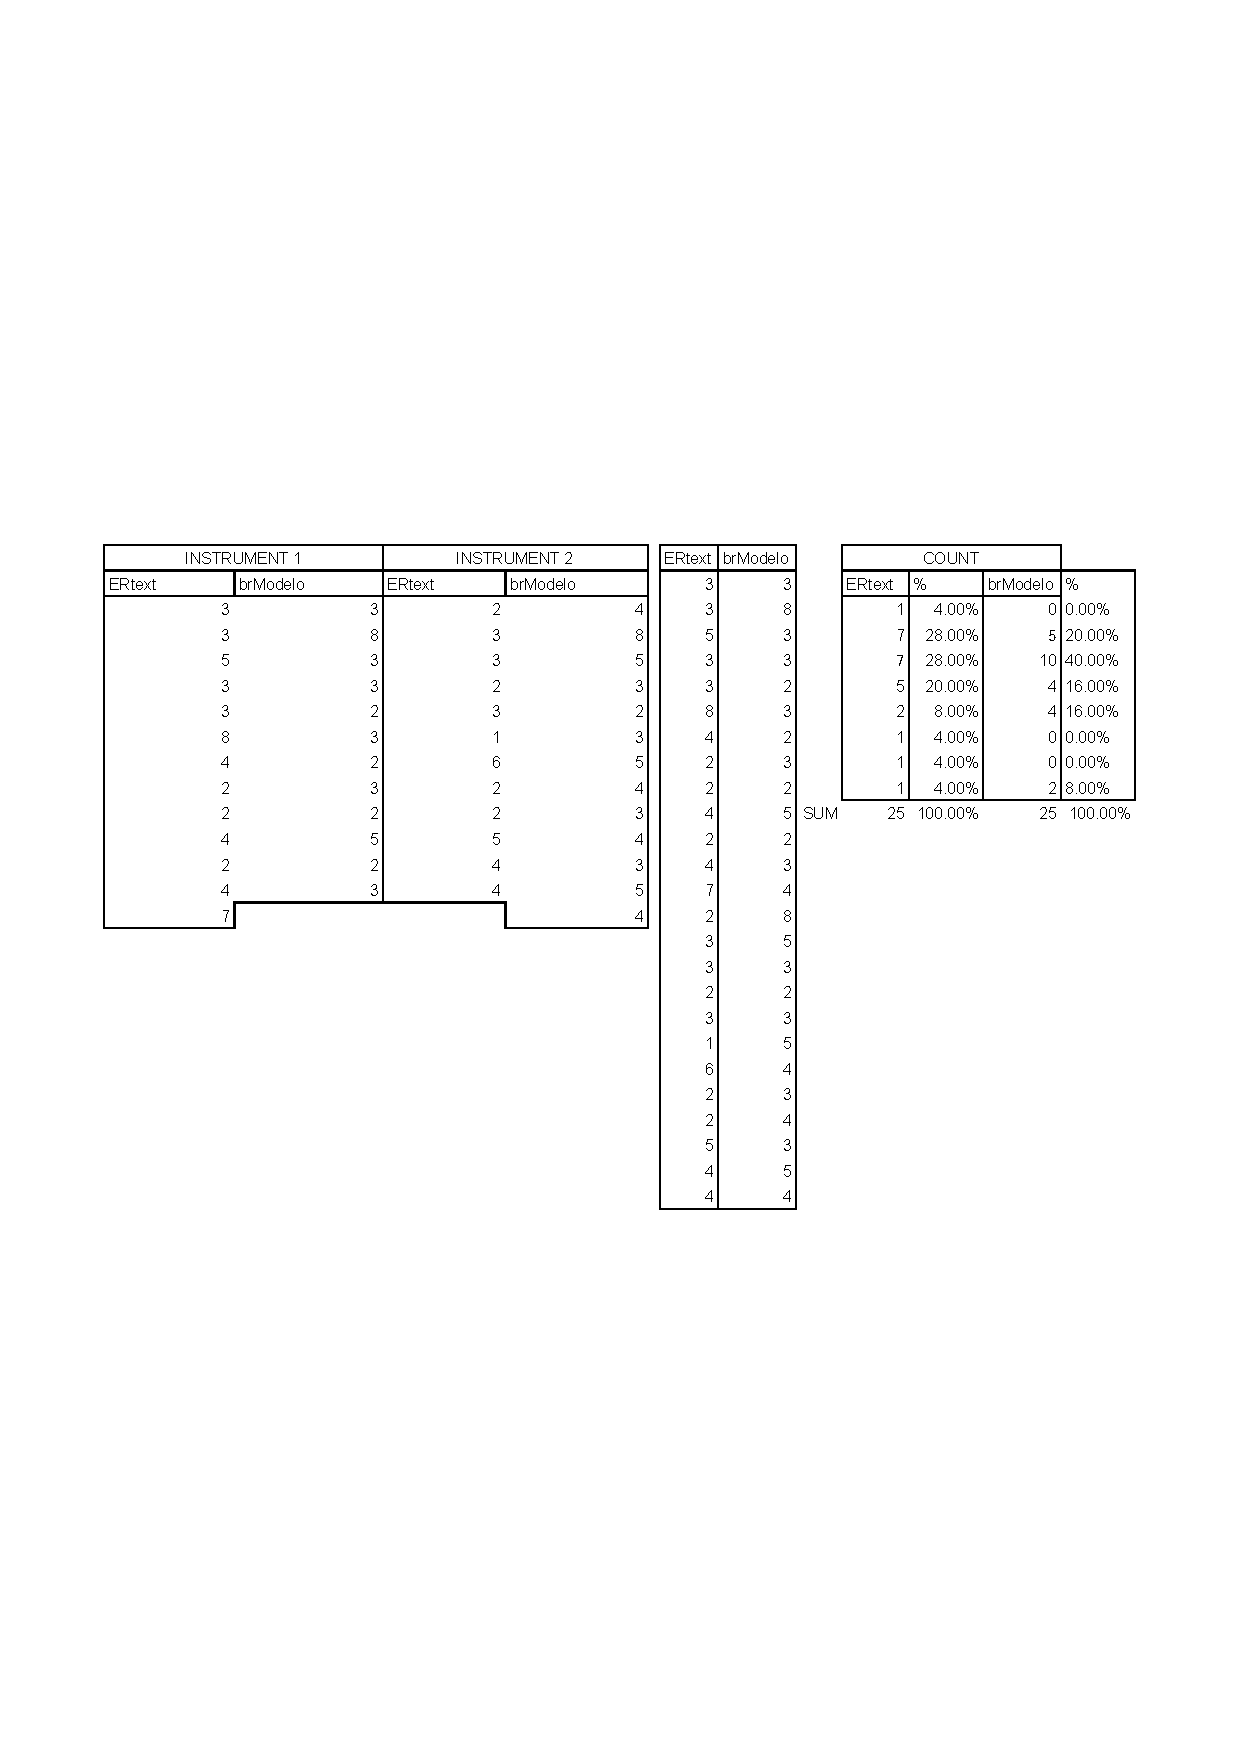
\includegraphics[]{postextuais/appendix/EX2-Results-Emocards.pdf}
    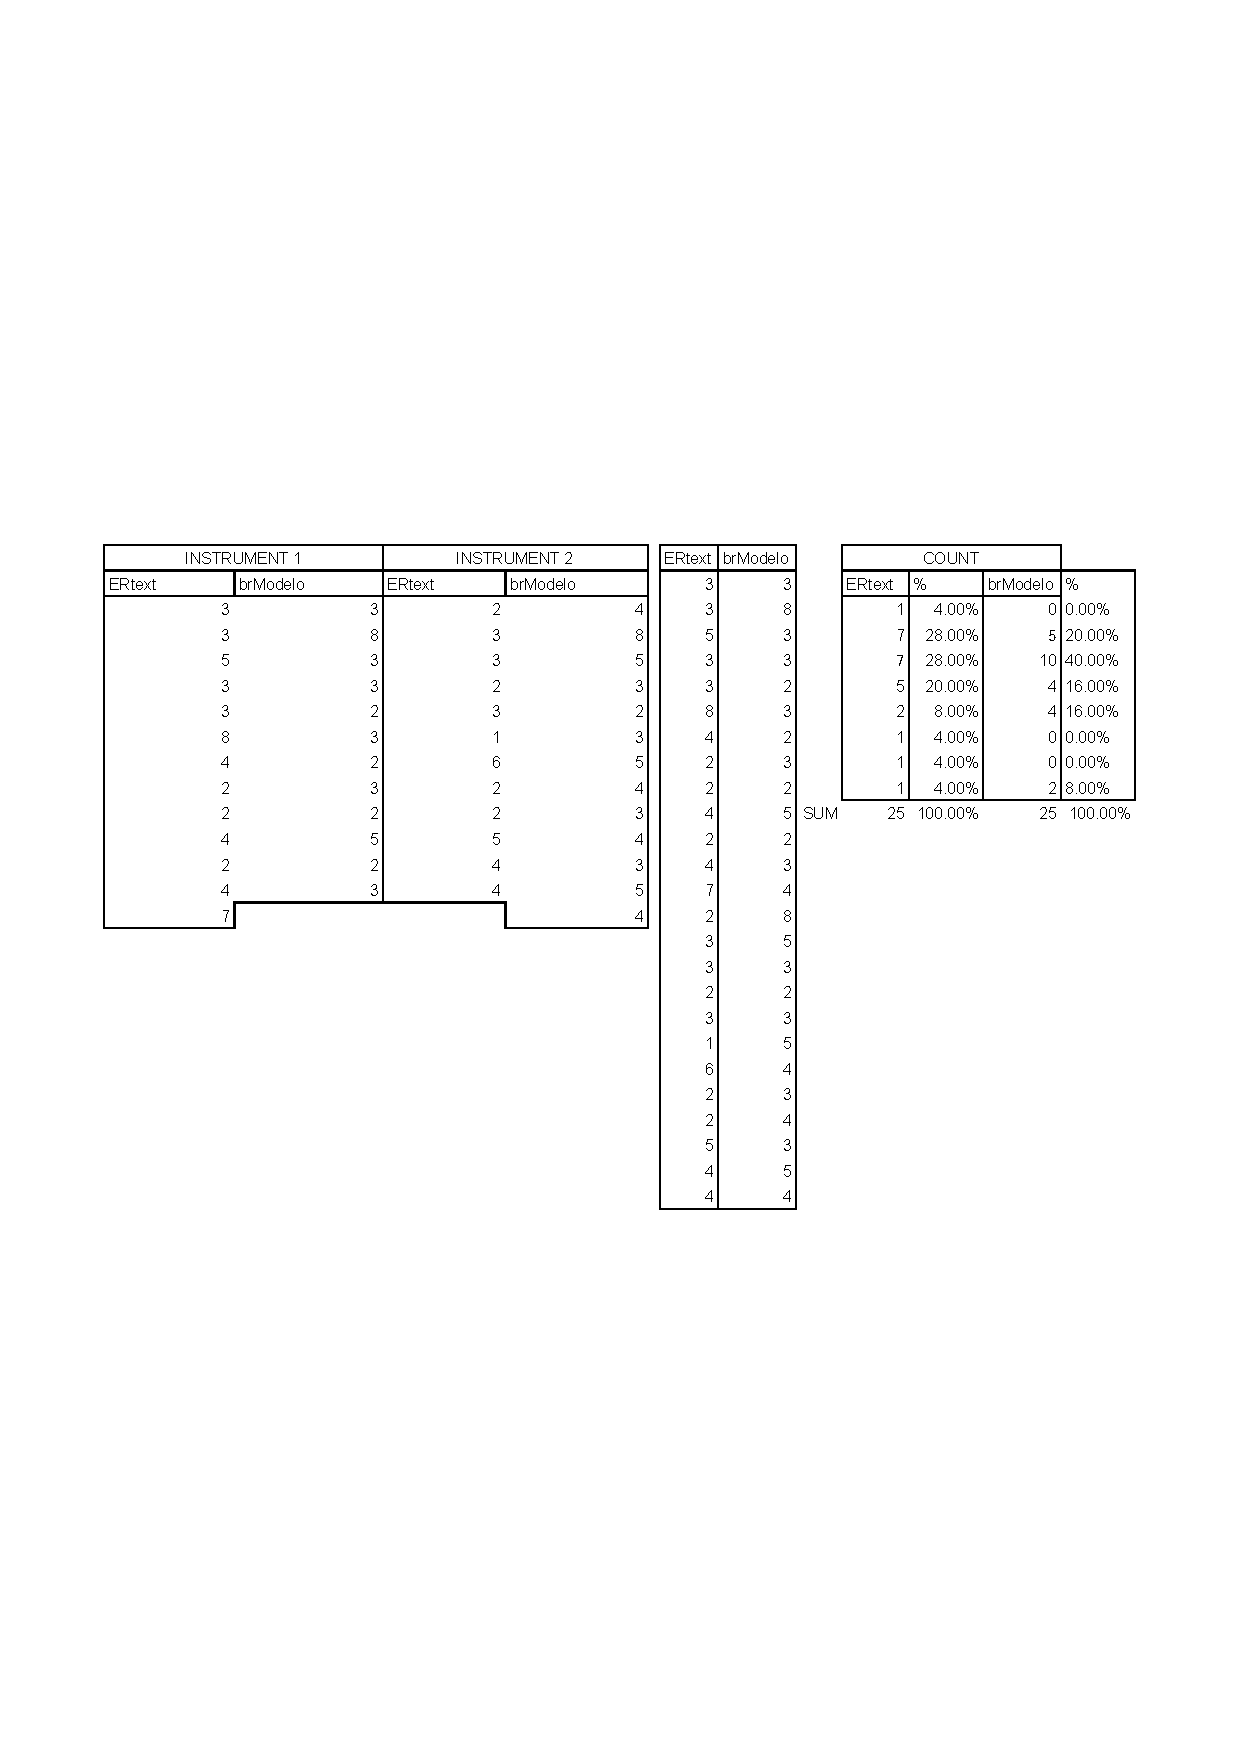
\includepdf[pages=-, frame=false, scale=0.90]{postextuais/appendix/EX2-Results-Emocards.pdf}
    \caption{EX2 - Emocards.}
    \label{fig:ex2Emocards}
\end{figure}



% ==============================================================================
\chapter{Experiment 3 (EX3)}
% ==============================================================================

\begin{figure}
    \centering
    % 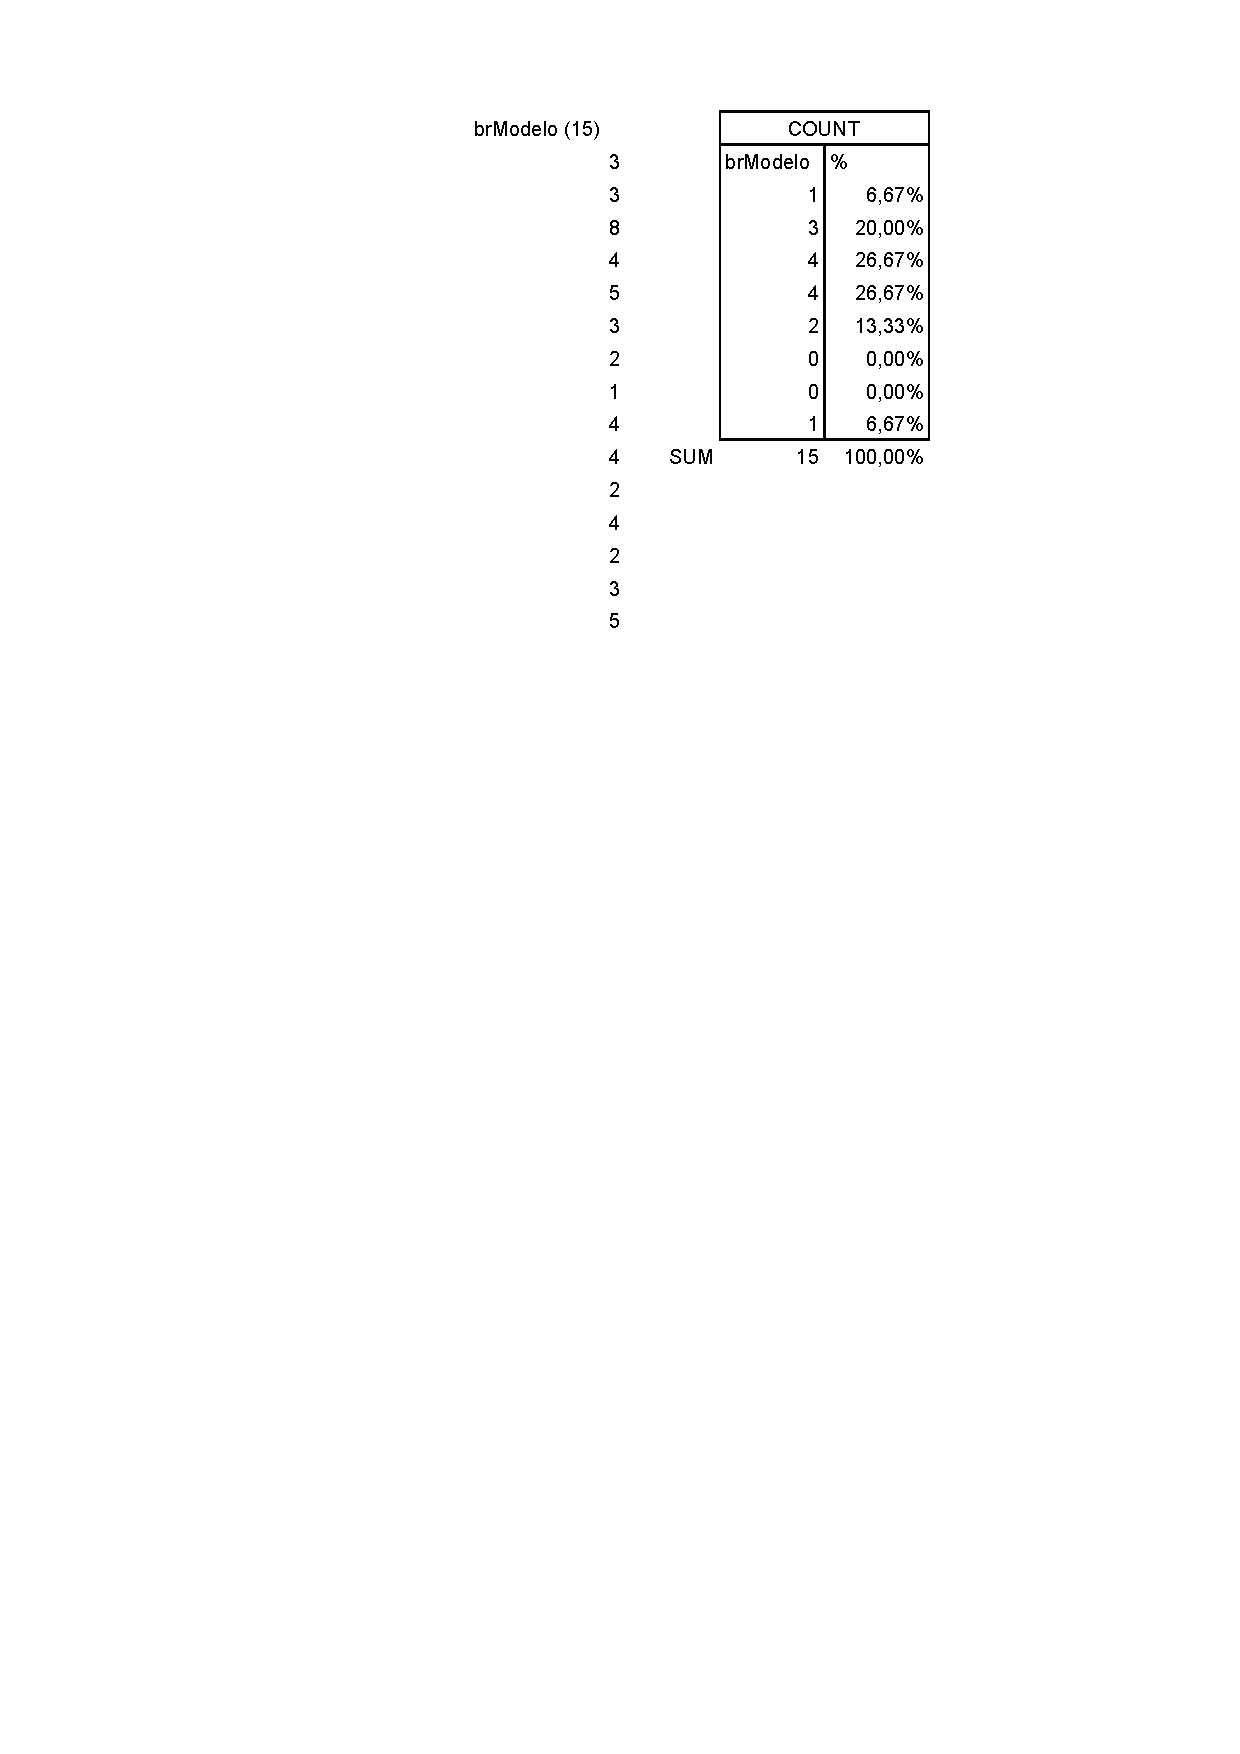
\includegraphics[]{postextuais/appendix/EX3- Emocards-brModelo.pdf}
    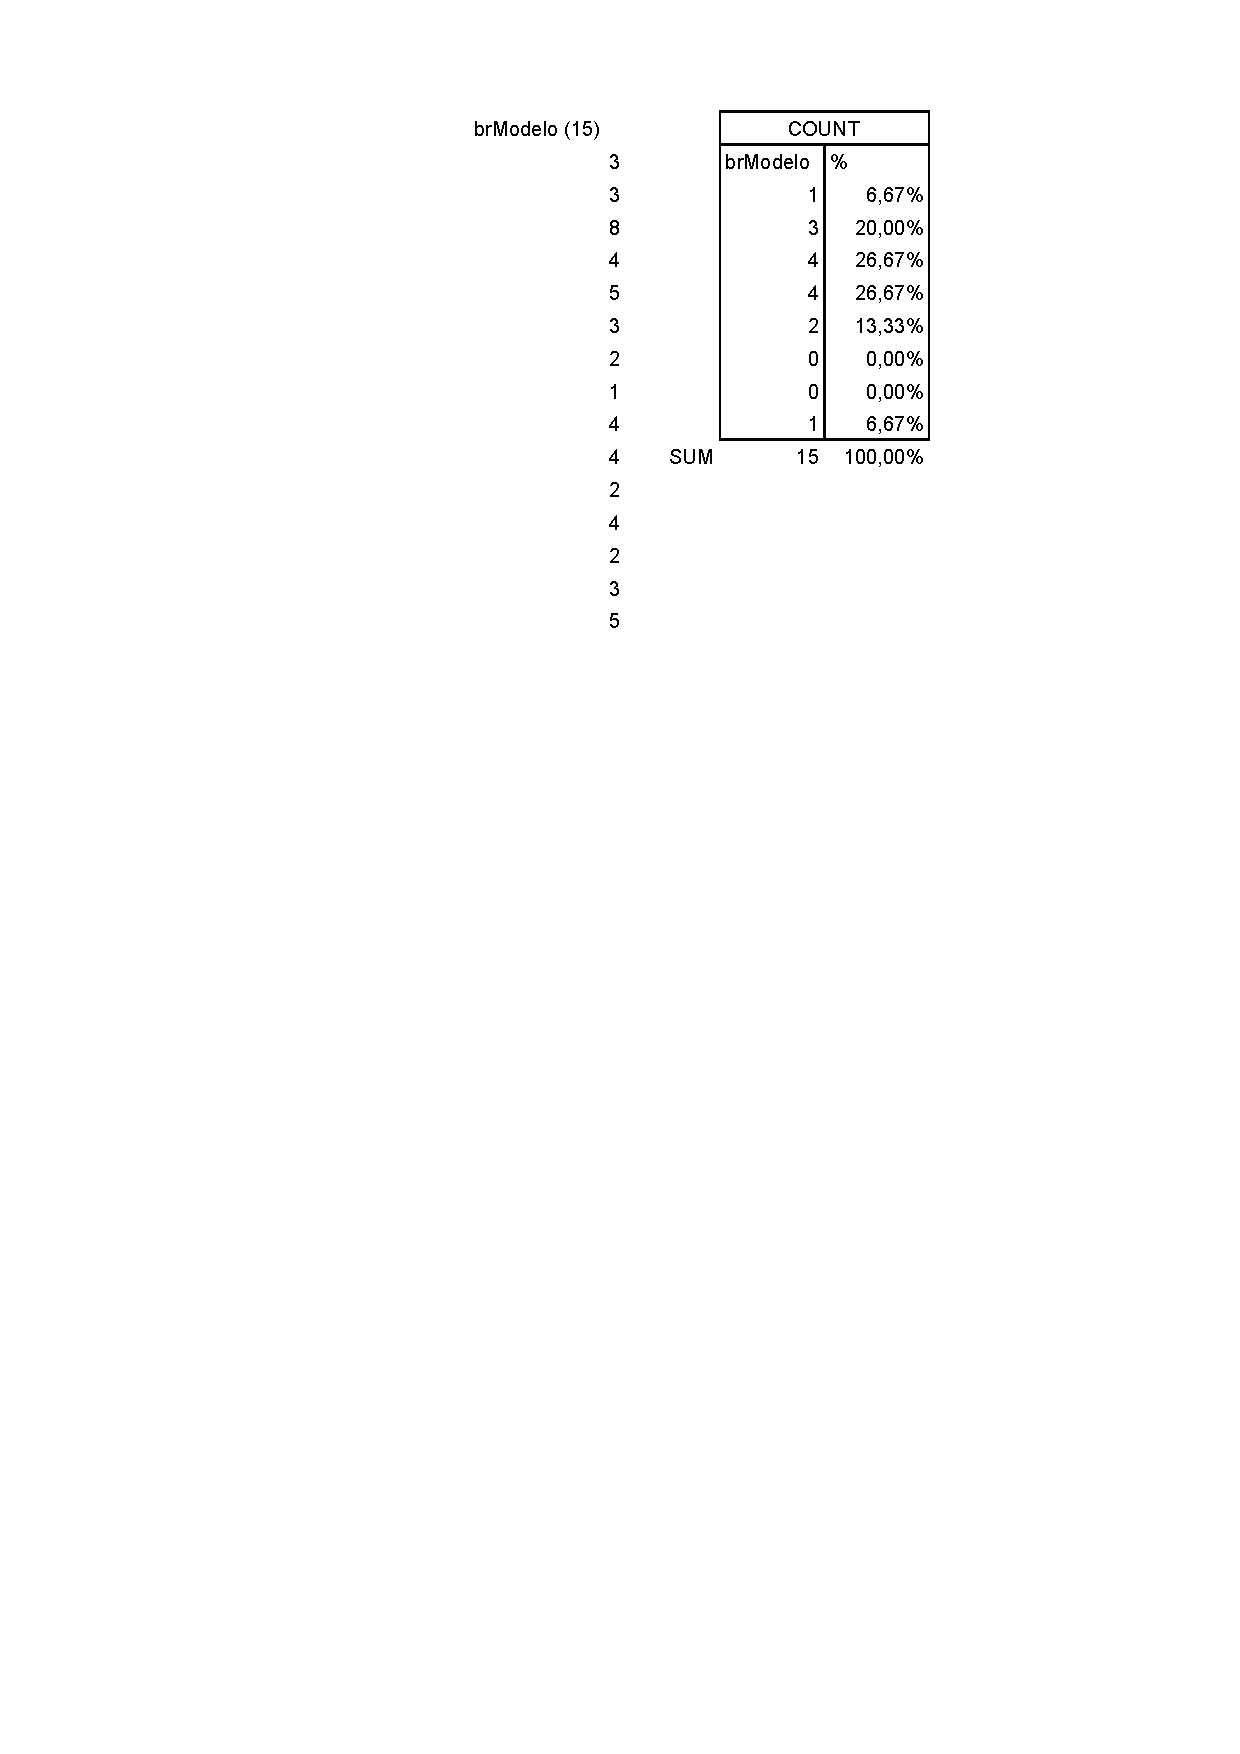
\includepdf[pages=-, frame=false, scale=0.90]{postextuais/appendix/EX3- Emocards-brModelo.pdf}
    \caption{EX3 - Emocards - brModelo.}
    \label{fig:ex3EmocardsbrModelo}
\end{figure}

\newpage

\begin{figure}
    \centering
    % 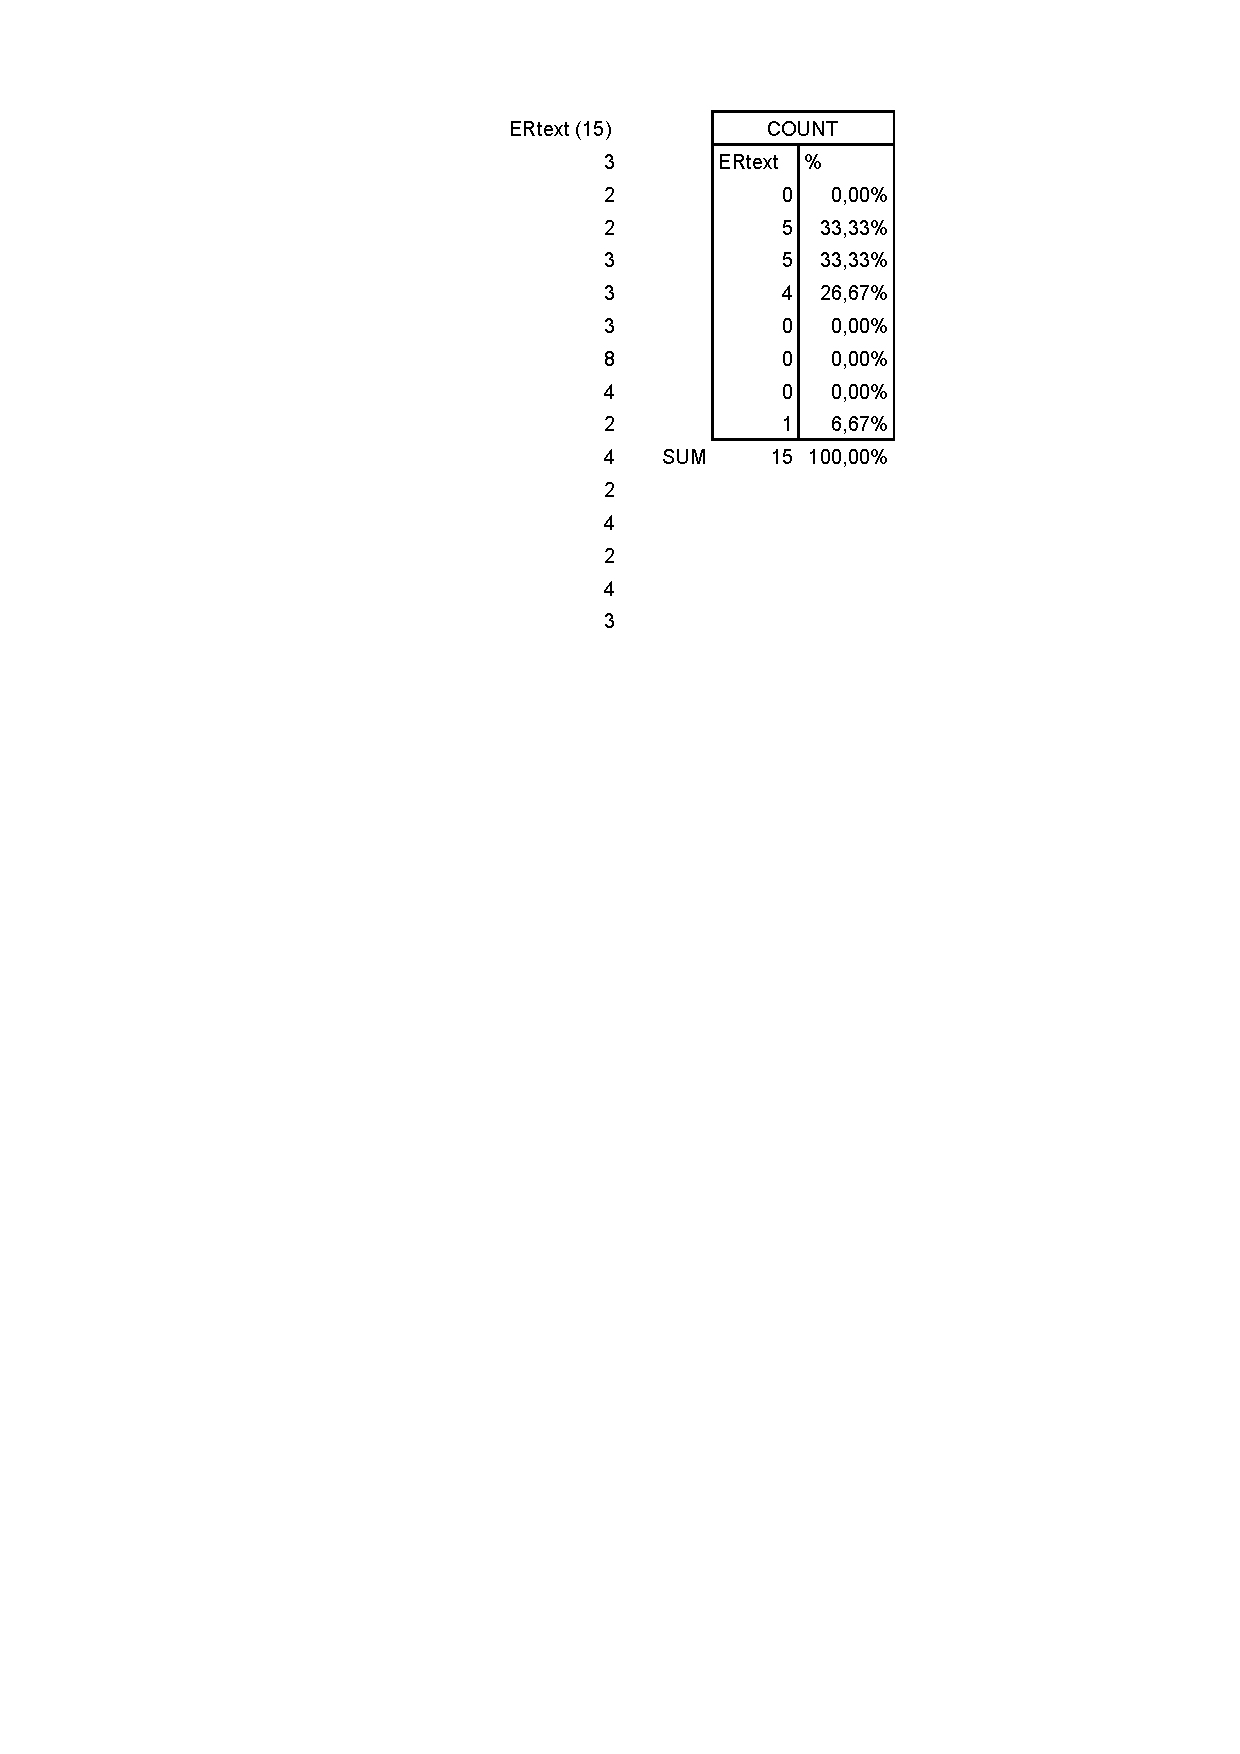
\includegraphics[]{postextuais/appendix/EX3- Emocards-ERtext.pdf}
    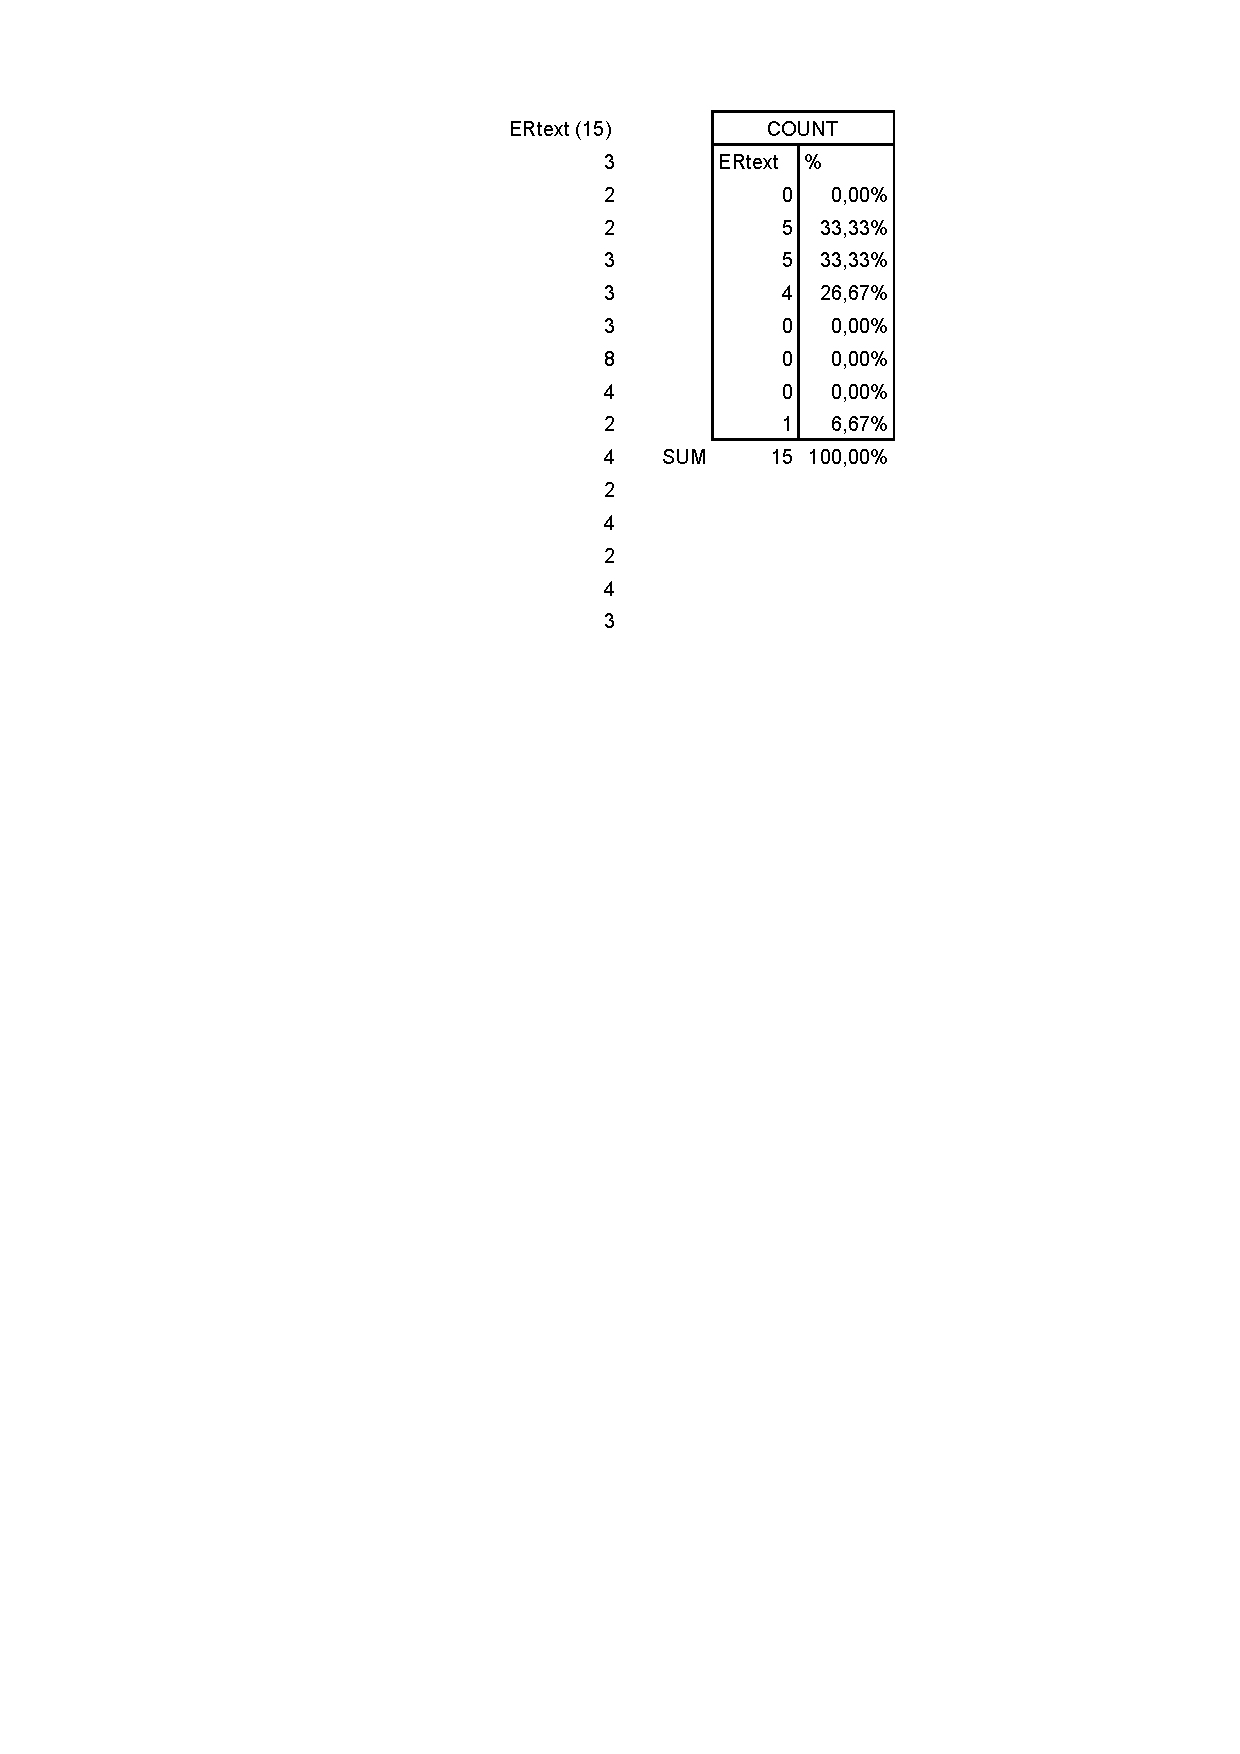
\includepdf[pages=-, frame=false, scale=0.90]{postextuais/appendix/EX3- Emocards-ERtext.pdf}
    \caption{EX3 - Emocards - ERtext.}
    \label{fig:ex3EmocardsERtext}
\end{figure}

\newpage

\begin{figure}
    \centering
    % 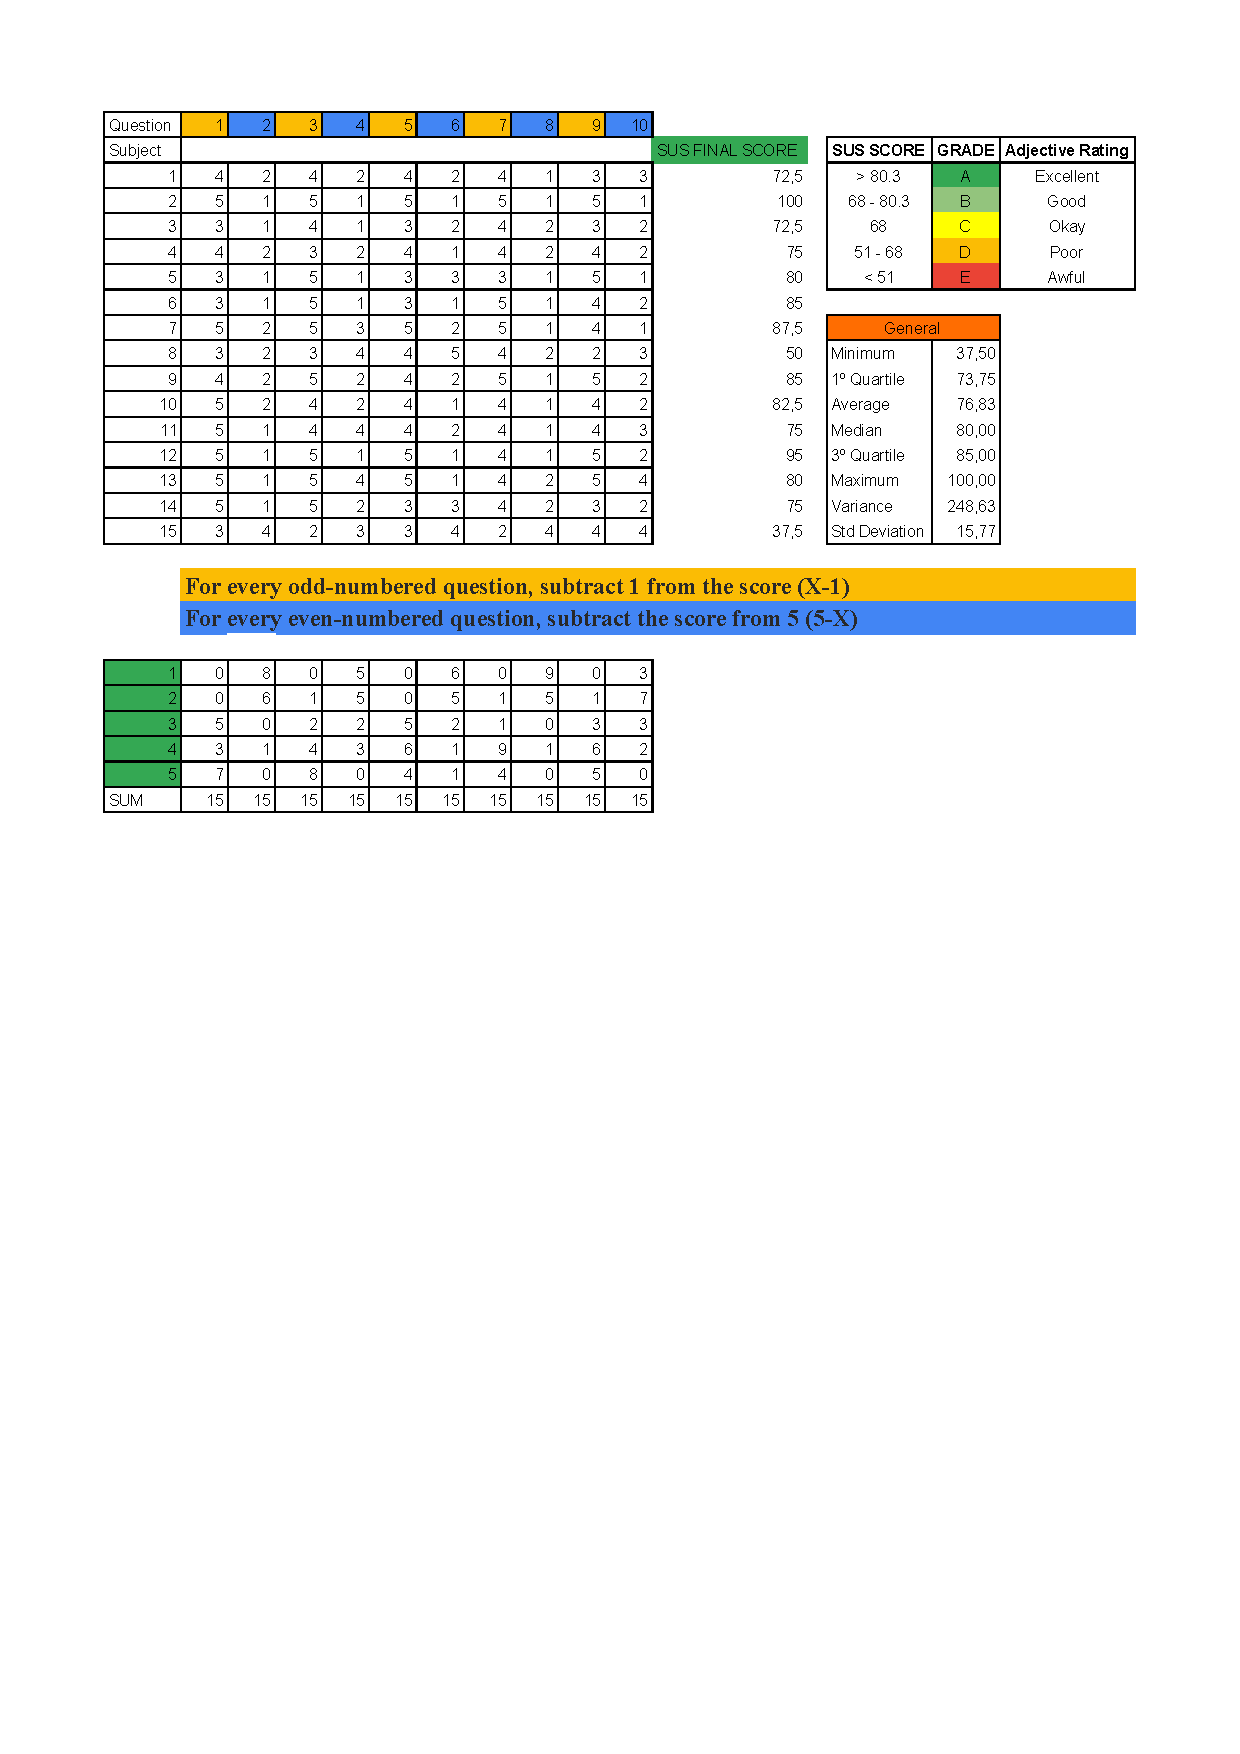
\includegraphics[]{postextuais/appendix/EX3-SUS-brModelo.pdf}
    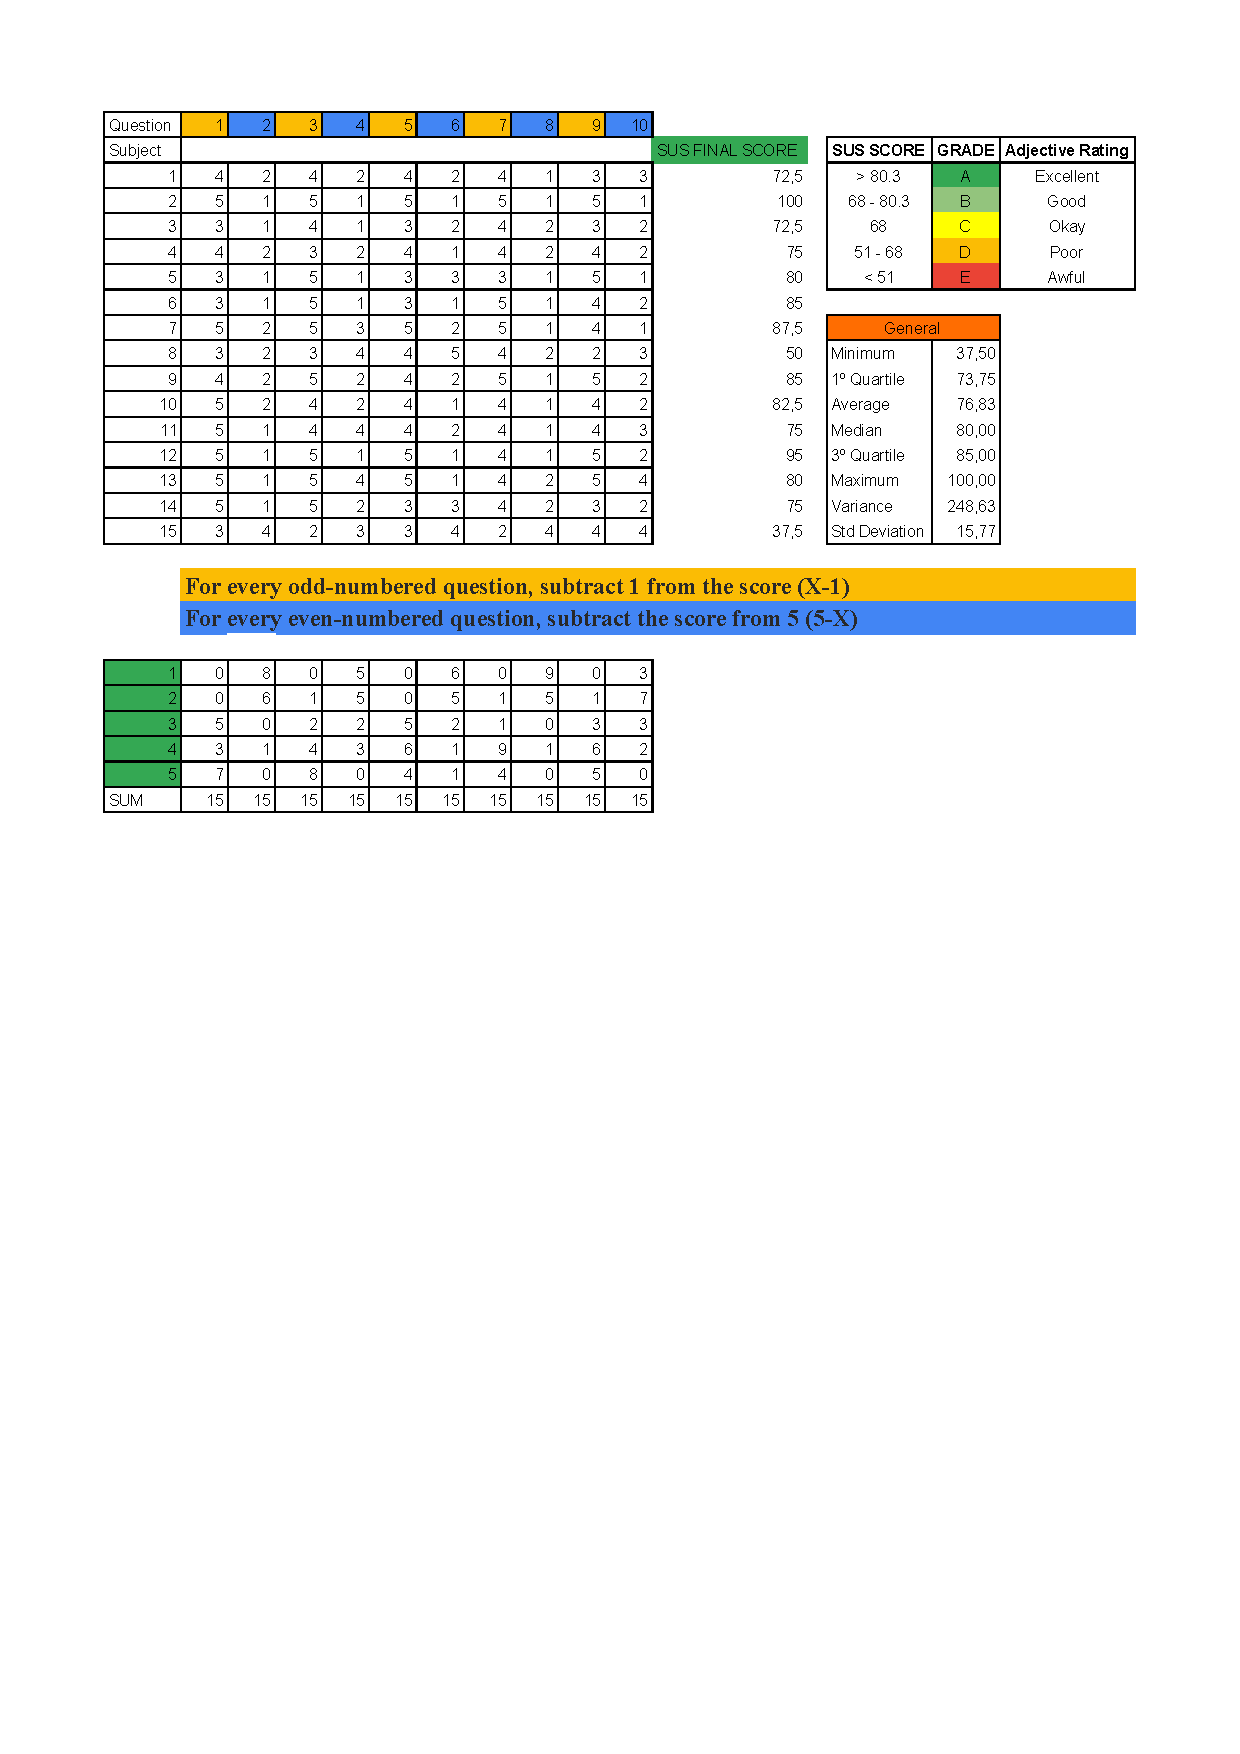
\includepdf[pages=-, frame=false, scale=0.90]{postextuais/appendix/EX3-SUS-brModelo.pdf}
    \caption{EX3 - SUS - brModelo.}
    \label{fig:ex3EmocardsERtext}
\end{figure}

\newpage

\begin{figure}
    \centering
    % 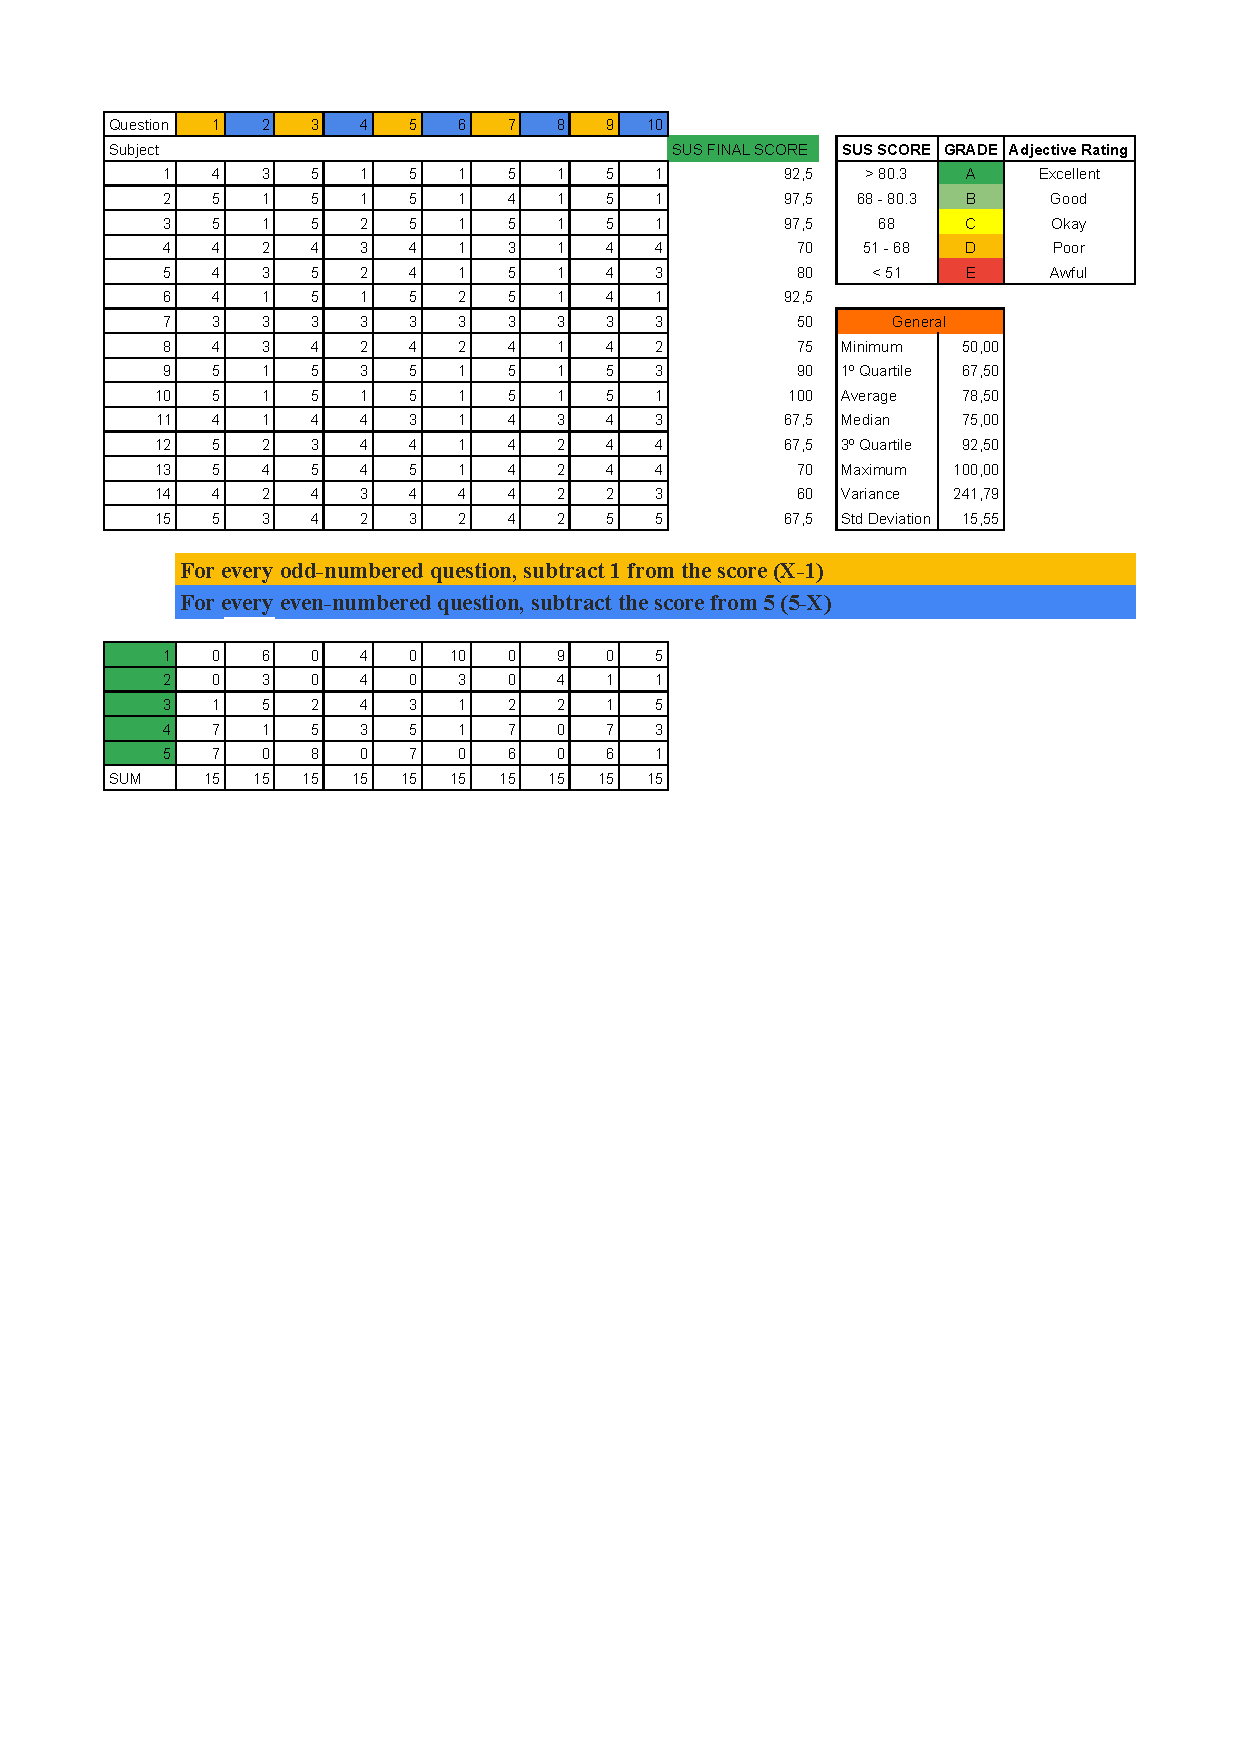
\includegraphics[]{postextuais/appendix/EX3-SUS-ERtext.pdf}
    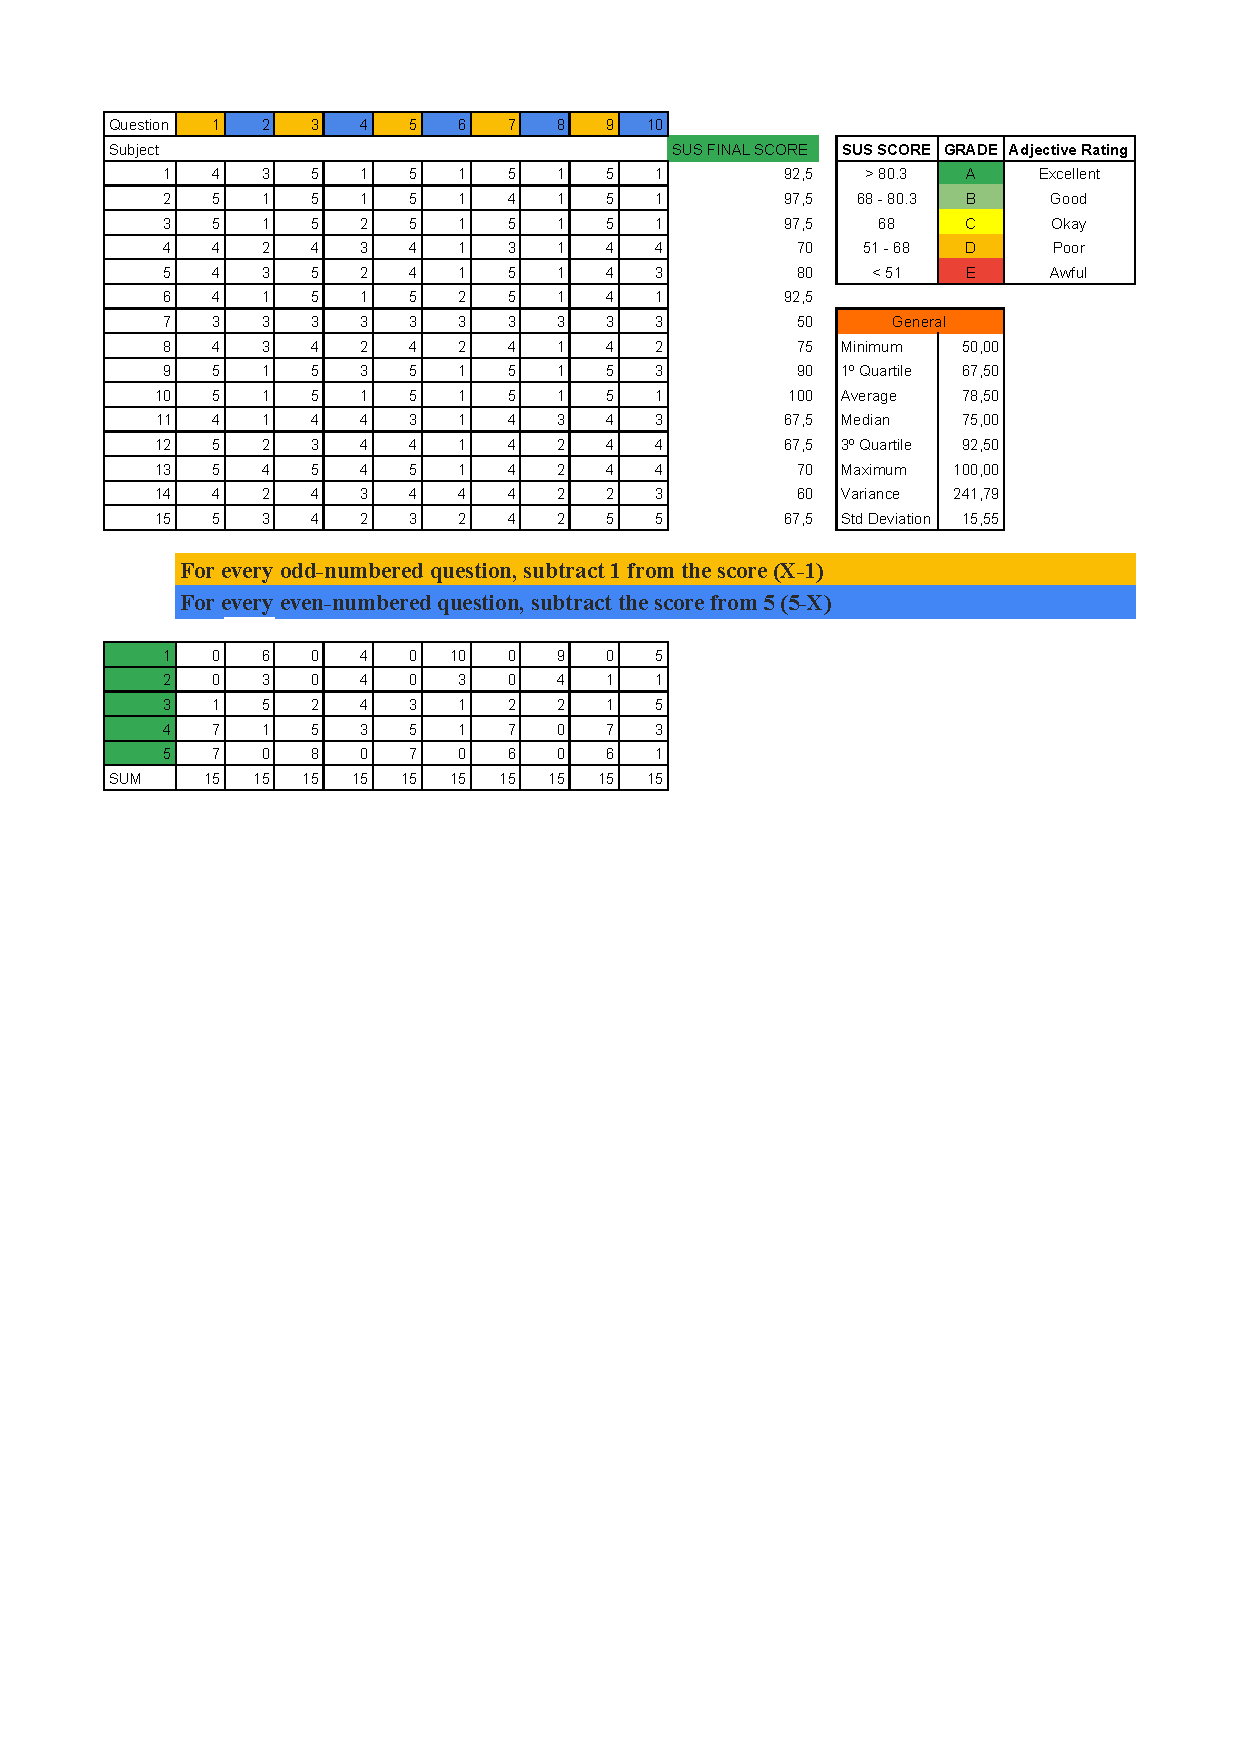
\includepdf[pages=-, frame=false, scale=0.90]{postextuais/appendix/EX3-SUS-ERtext.pdf}
    \caption{EX3 - SUS - ERtext.}
    \label{fig:ex3EmocardsERtext}
\end{figure}

\end{apendicesenv}
